% !TeX root = ../main.tex
% Add the above to each chapter to make compiling the PDF easier in some editors.

\chapter{Results}\label{chapter:results}

Due to the imbalanced nature of the datasets, in order to account for the rare classes macro recall is used as the main metric (section \ref{section:evaluation_metrics}).

%Todo: I have to add different captions for different figures here
\begin{figure}[htbp]
\centering
\captionsetup{format=plain}
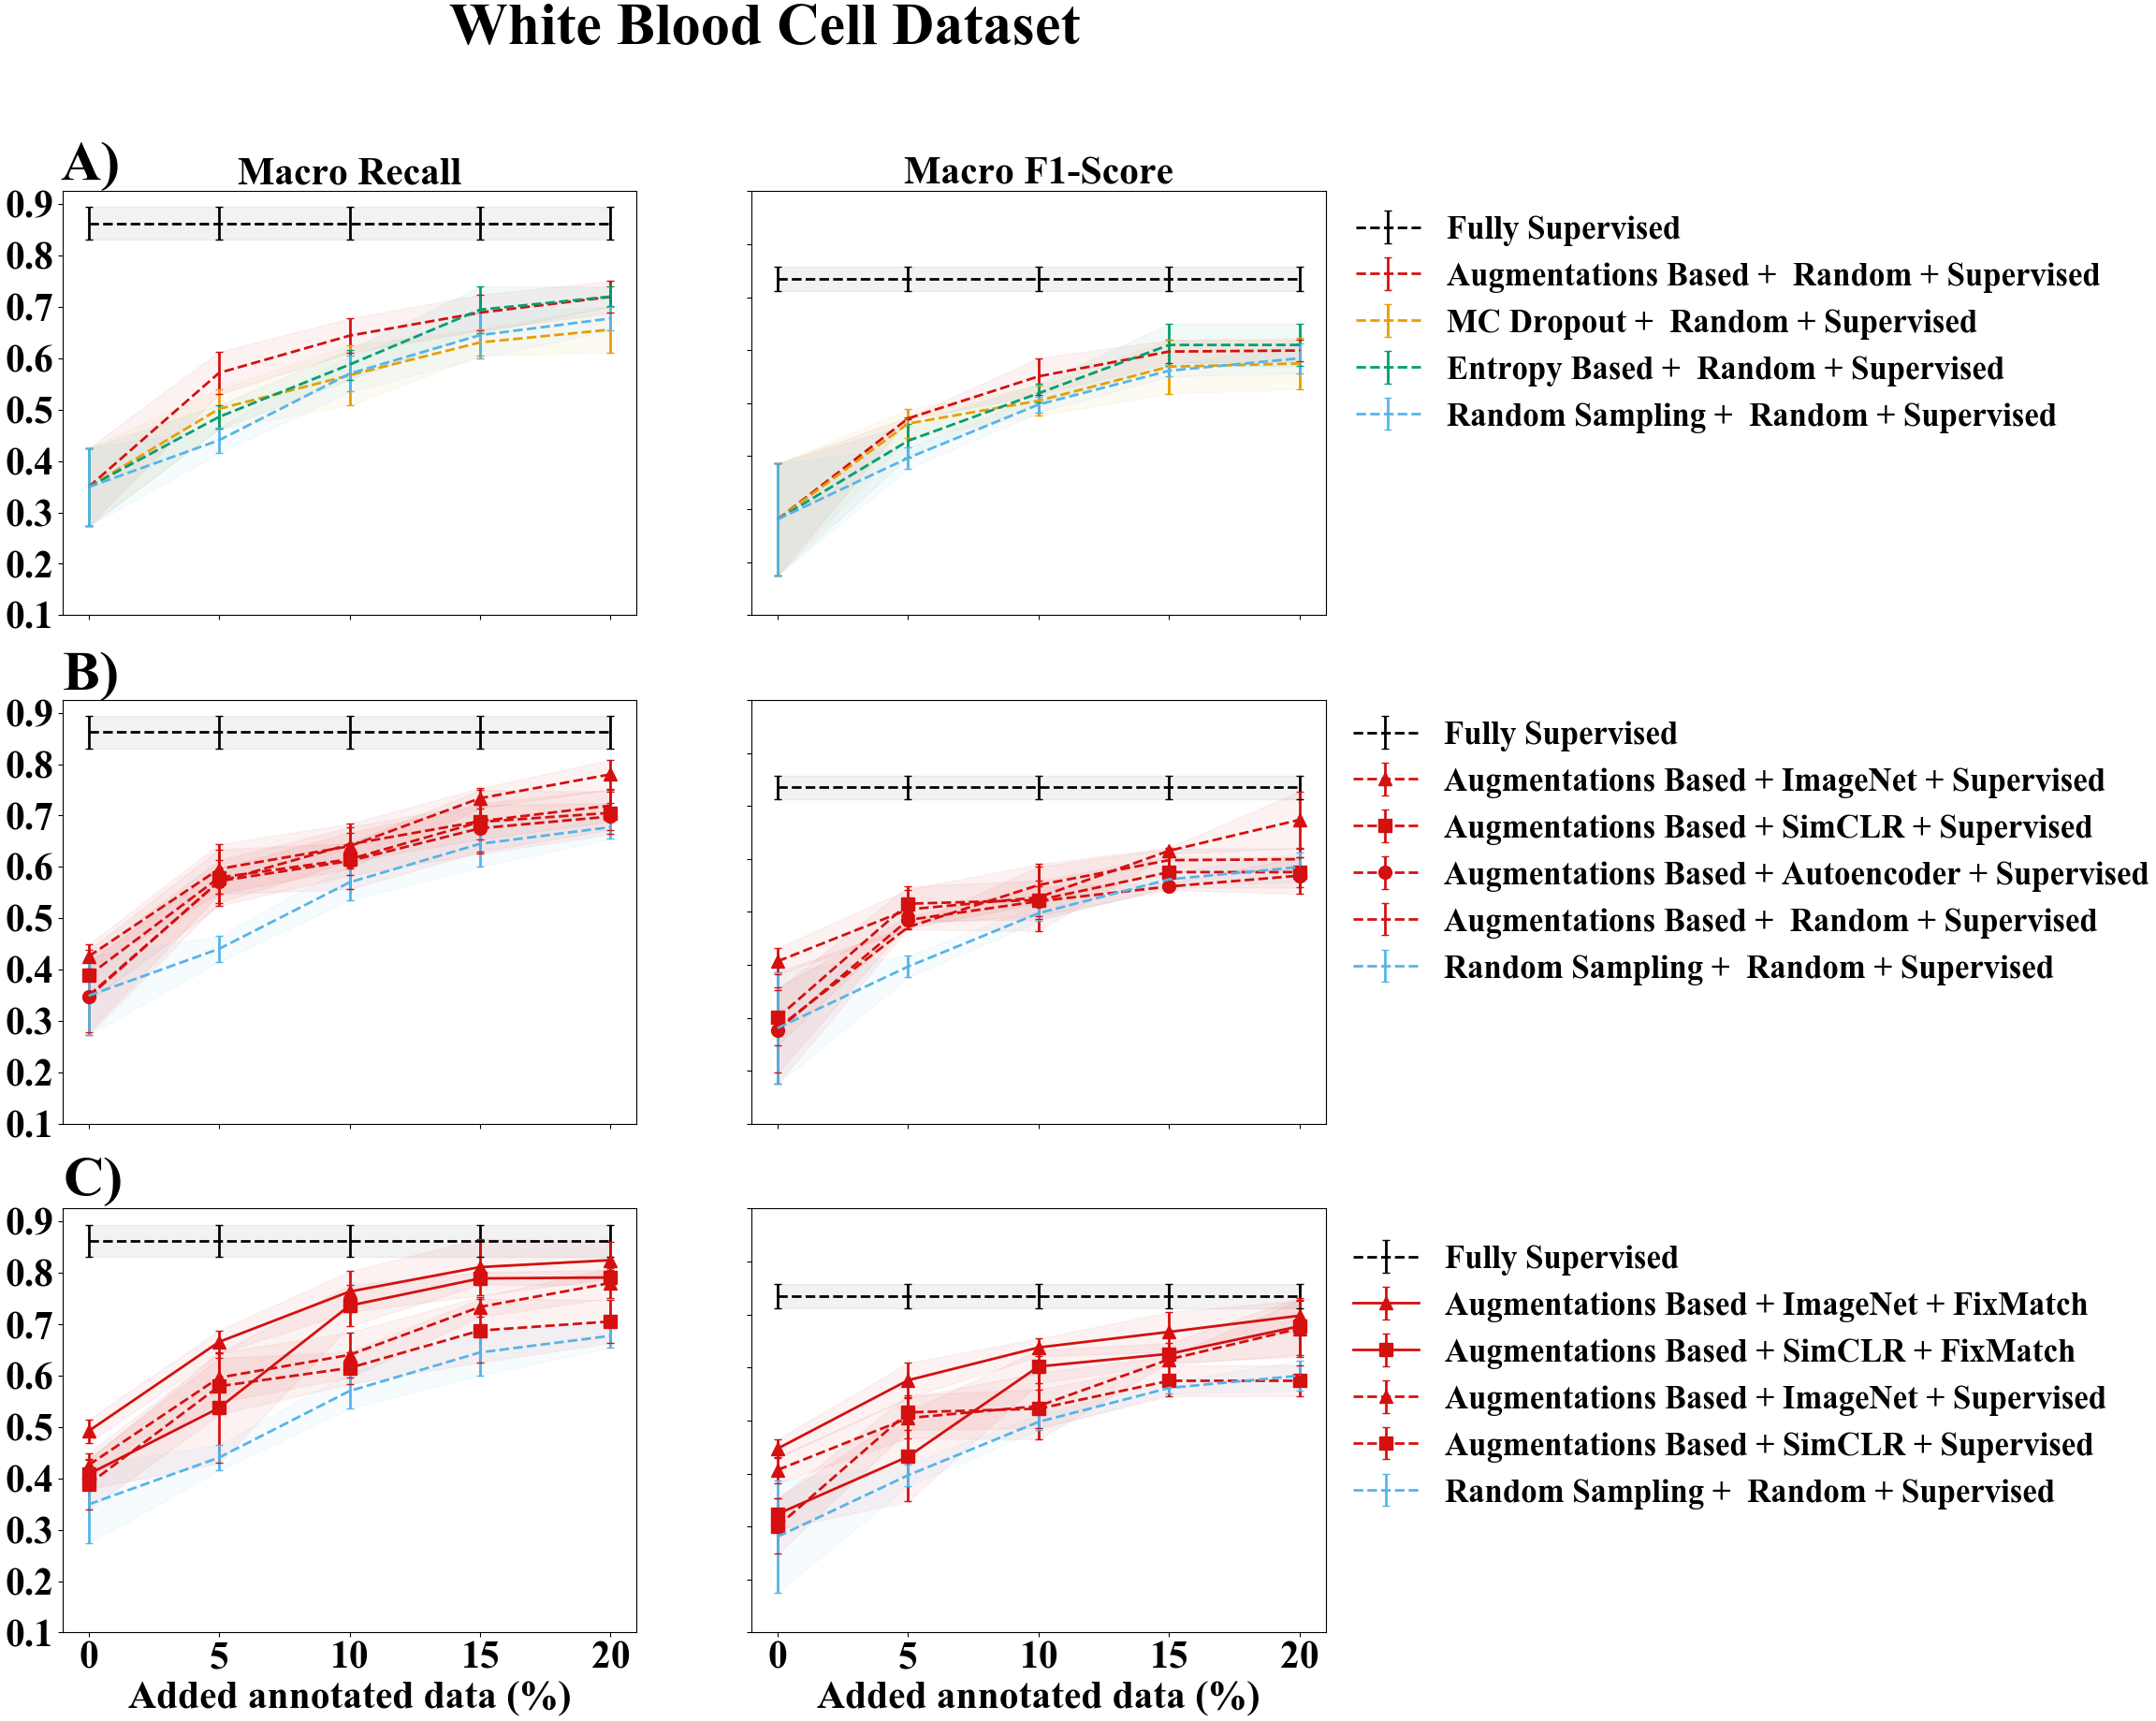
\includegraphics[width=\textwidth]{figures/fig_2_white_recall_f1.png}
\caption[Macro recall and macro f1-score on white blood cell dataset]{\textbf{Macro recall and macro f1-score on white blood cell dataset}. In the white blood cell dataset, the combination of augmentation-based sampling, pre-trained ImageNet weights pre-training and semi-supervised learning using FixMatch results in a performance which converges to fully-supervised learning. (A) Macro recall and macro f1-score is depicted for 3 active learning algorithms. The dashed red line represents augmentation-based sampling, dashed green line represents the entropy-based sampling, dashed yellow line shows MC-dropout and the dashed blue line show random sampling. 1\% of data is used initially and 5\% of the total data is added at every active learning iteration (B) The best performing active learning algorithm in terms of Macro Recall from A is augmentation-based sampling. It is chosen for making a comparison between different pre-training methods i.e., pre-trained ImageNet weights are shown with triangle markers, SimCLR with square markers and autoencoders are shown using circle markers. Random initialization with random sampling is shown as a dashed blue line. (C) For showing the effect of adding semi-supervised learning, FixMatch is used in conjunction with the best performing algorithms from B.}
\label{fig:fig_2_white_recall_f1}
\end{figure}

\begin{figure}[htbp]
\centering
\captionsetup{format=plain}
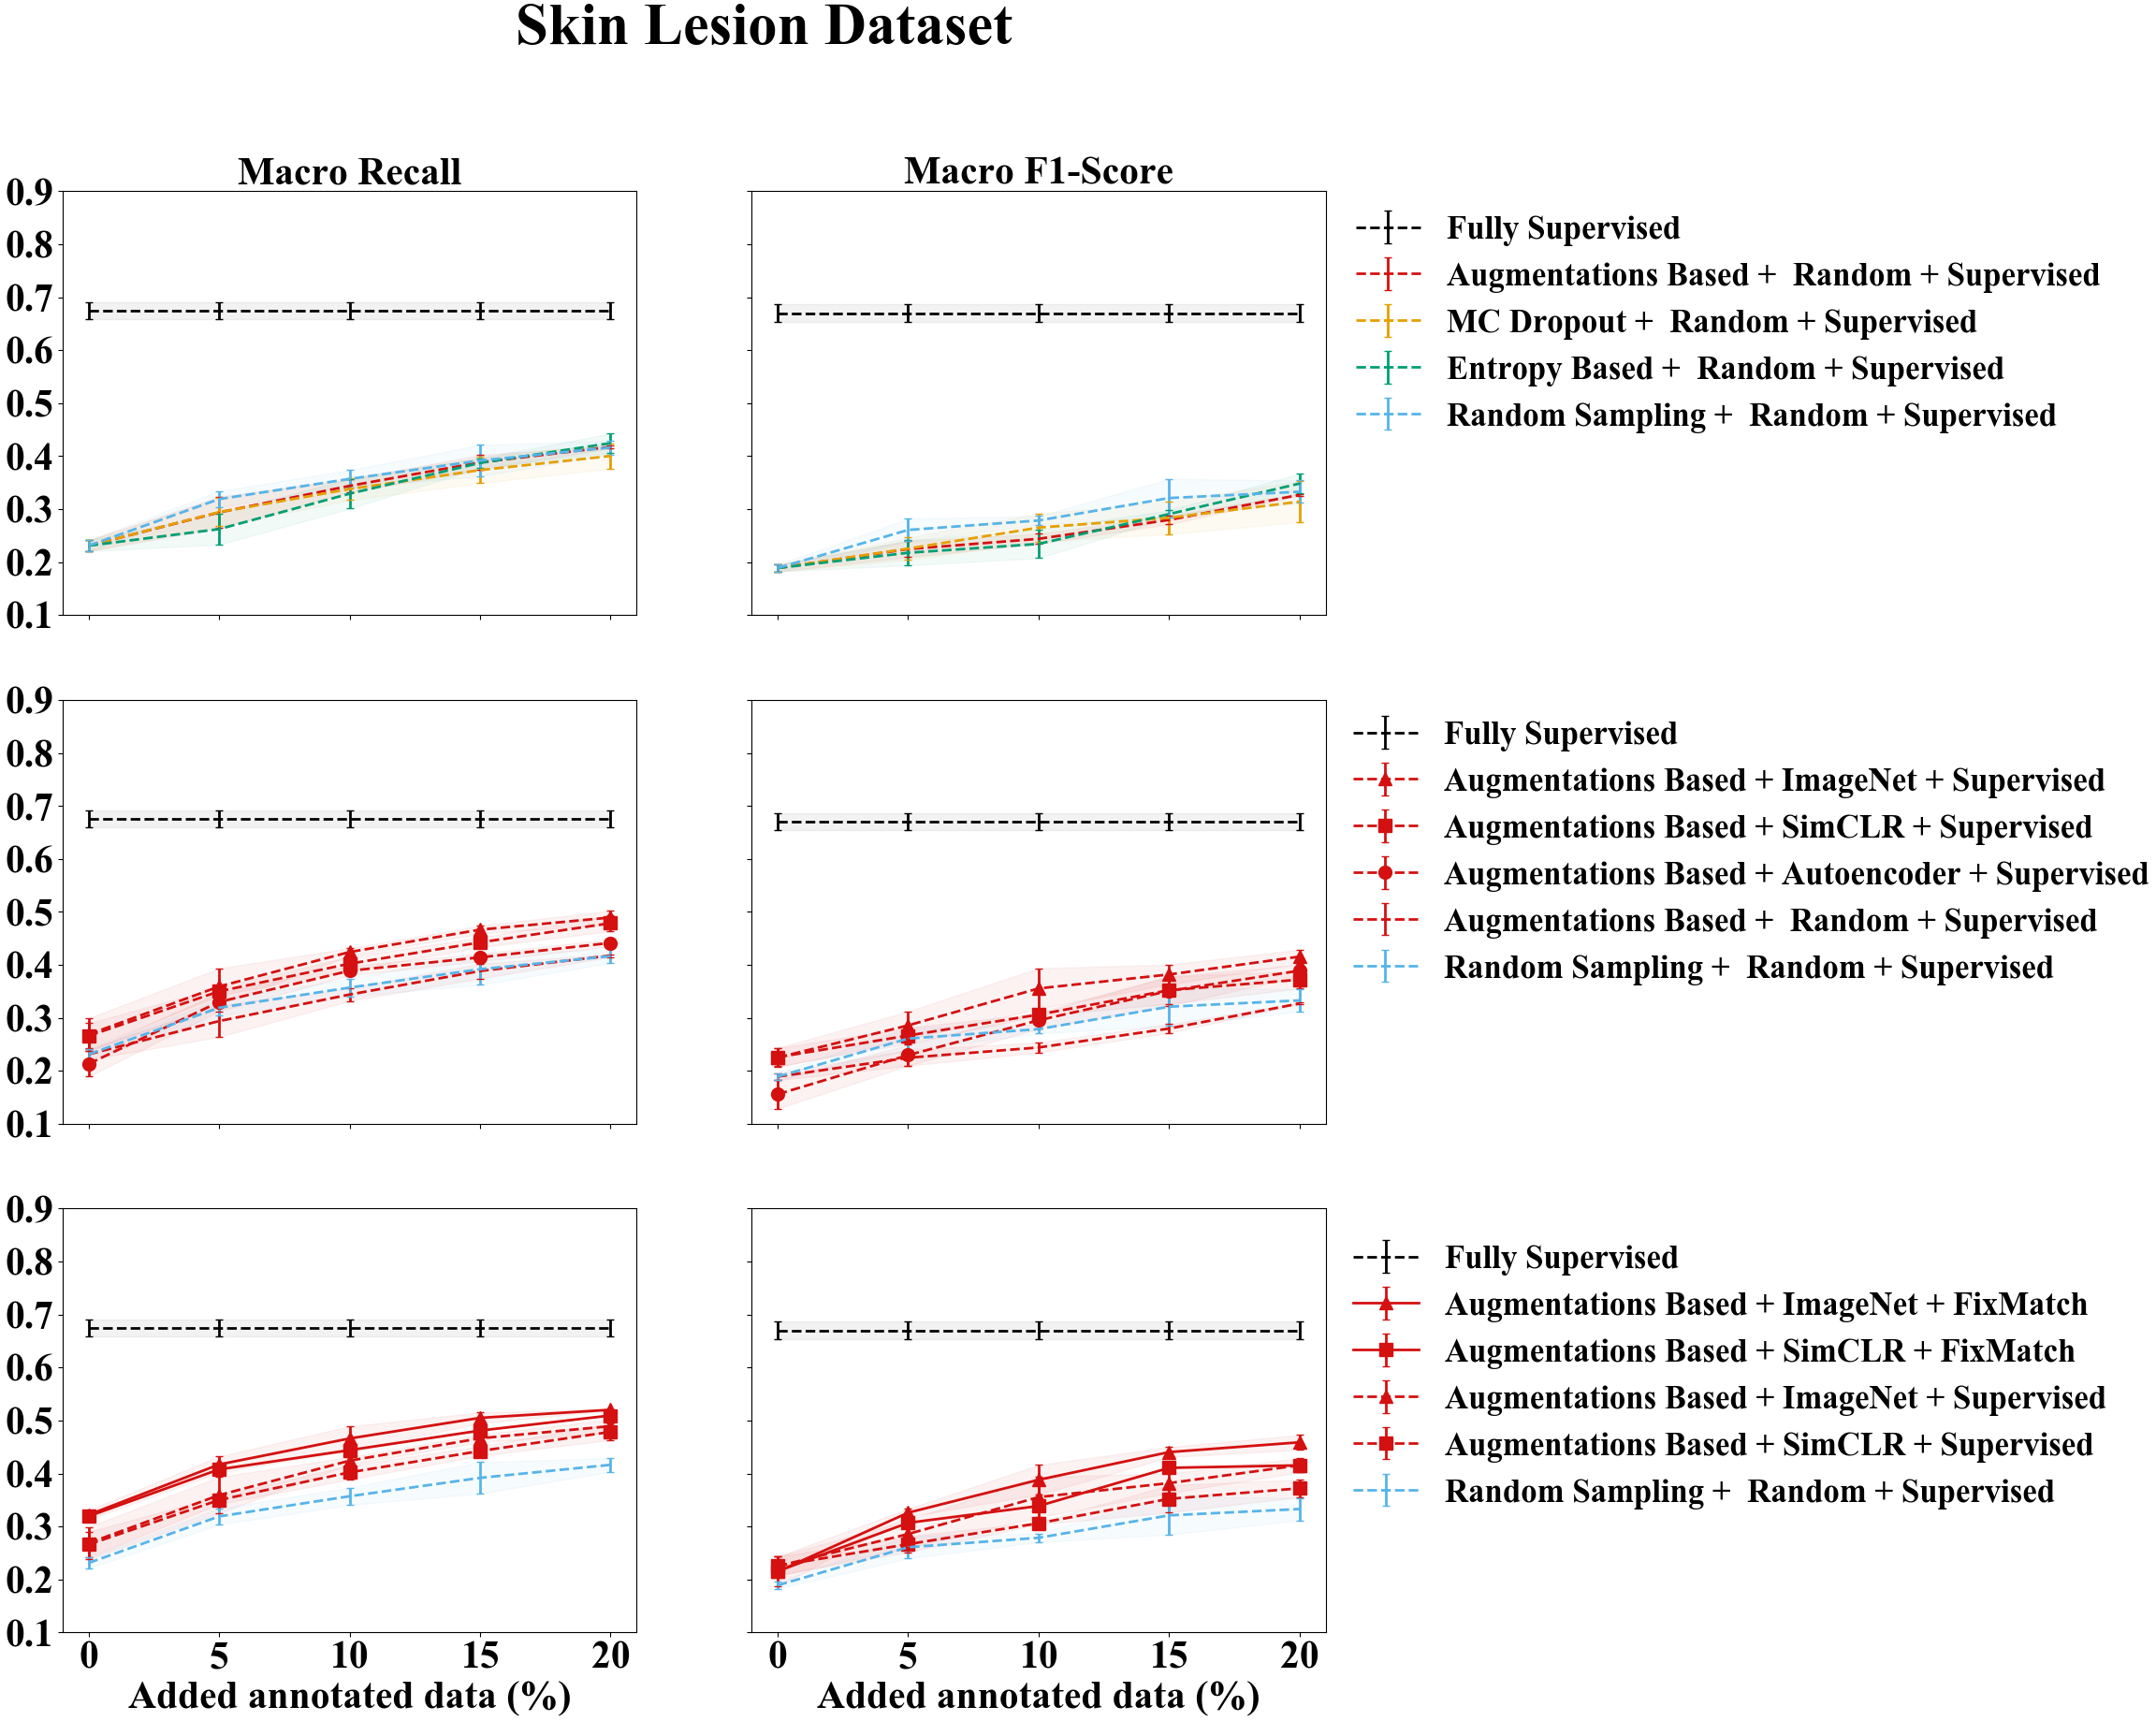
\includegraphics[width=\textwidth]{figures/fig_2_skin_recall_f1.png}
\caption[Macro recall and macro f1-score on skin lesion dataset]{\textbf{Macro recall and macro f1-score on skin lesion dataset}. In the skin lesion dataset, the combination of augmentation-based sampling, pre-trained ImageNet weights pre-training and semi-supervised learning is the best performing combination but the performance does not approach fully-supervised learning performance. (A) The figure depicts the macro recall and macro f1-score for the three active learning algorithms in addition to random sampling. All of the algorithms achieve similar performance for skin lesion dataset.(B) As mentioned in A, all active learning algorithms perform similarly. However, as augmentation is shown to be the best performing active learning algorithm (Table \ref{table:all_experiments_skin}) for skin lesion dataset during the extensive grid search, augmentation-based sampling's  performance for different pre-training methods has been shown. Pre-training using pre-trained ImageNet weights shows the best performance in terms of Macro Recall and Macro F1-score. (C) Lastly, to show the effect of semi-supervised learning, the best performing combination from B are selected and tested after the addition of FixMatch.}
\label{fig:fig_2_skin_recall_f1}
\end{figure}

\begin{figure}[htbp]
\centering
\captionsetup{format=plain}
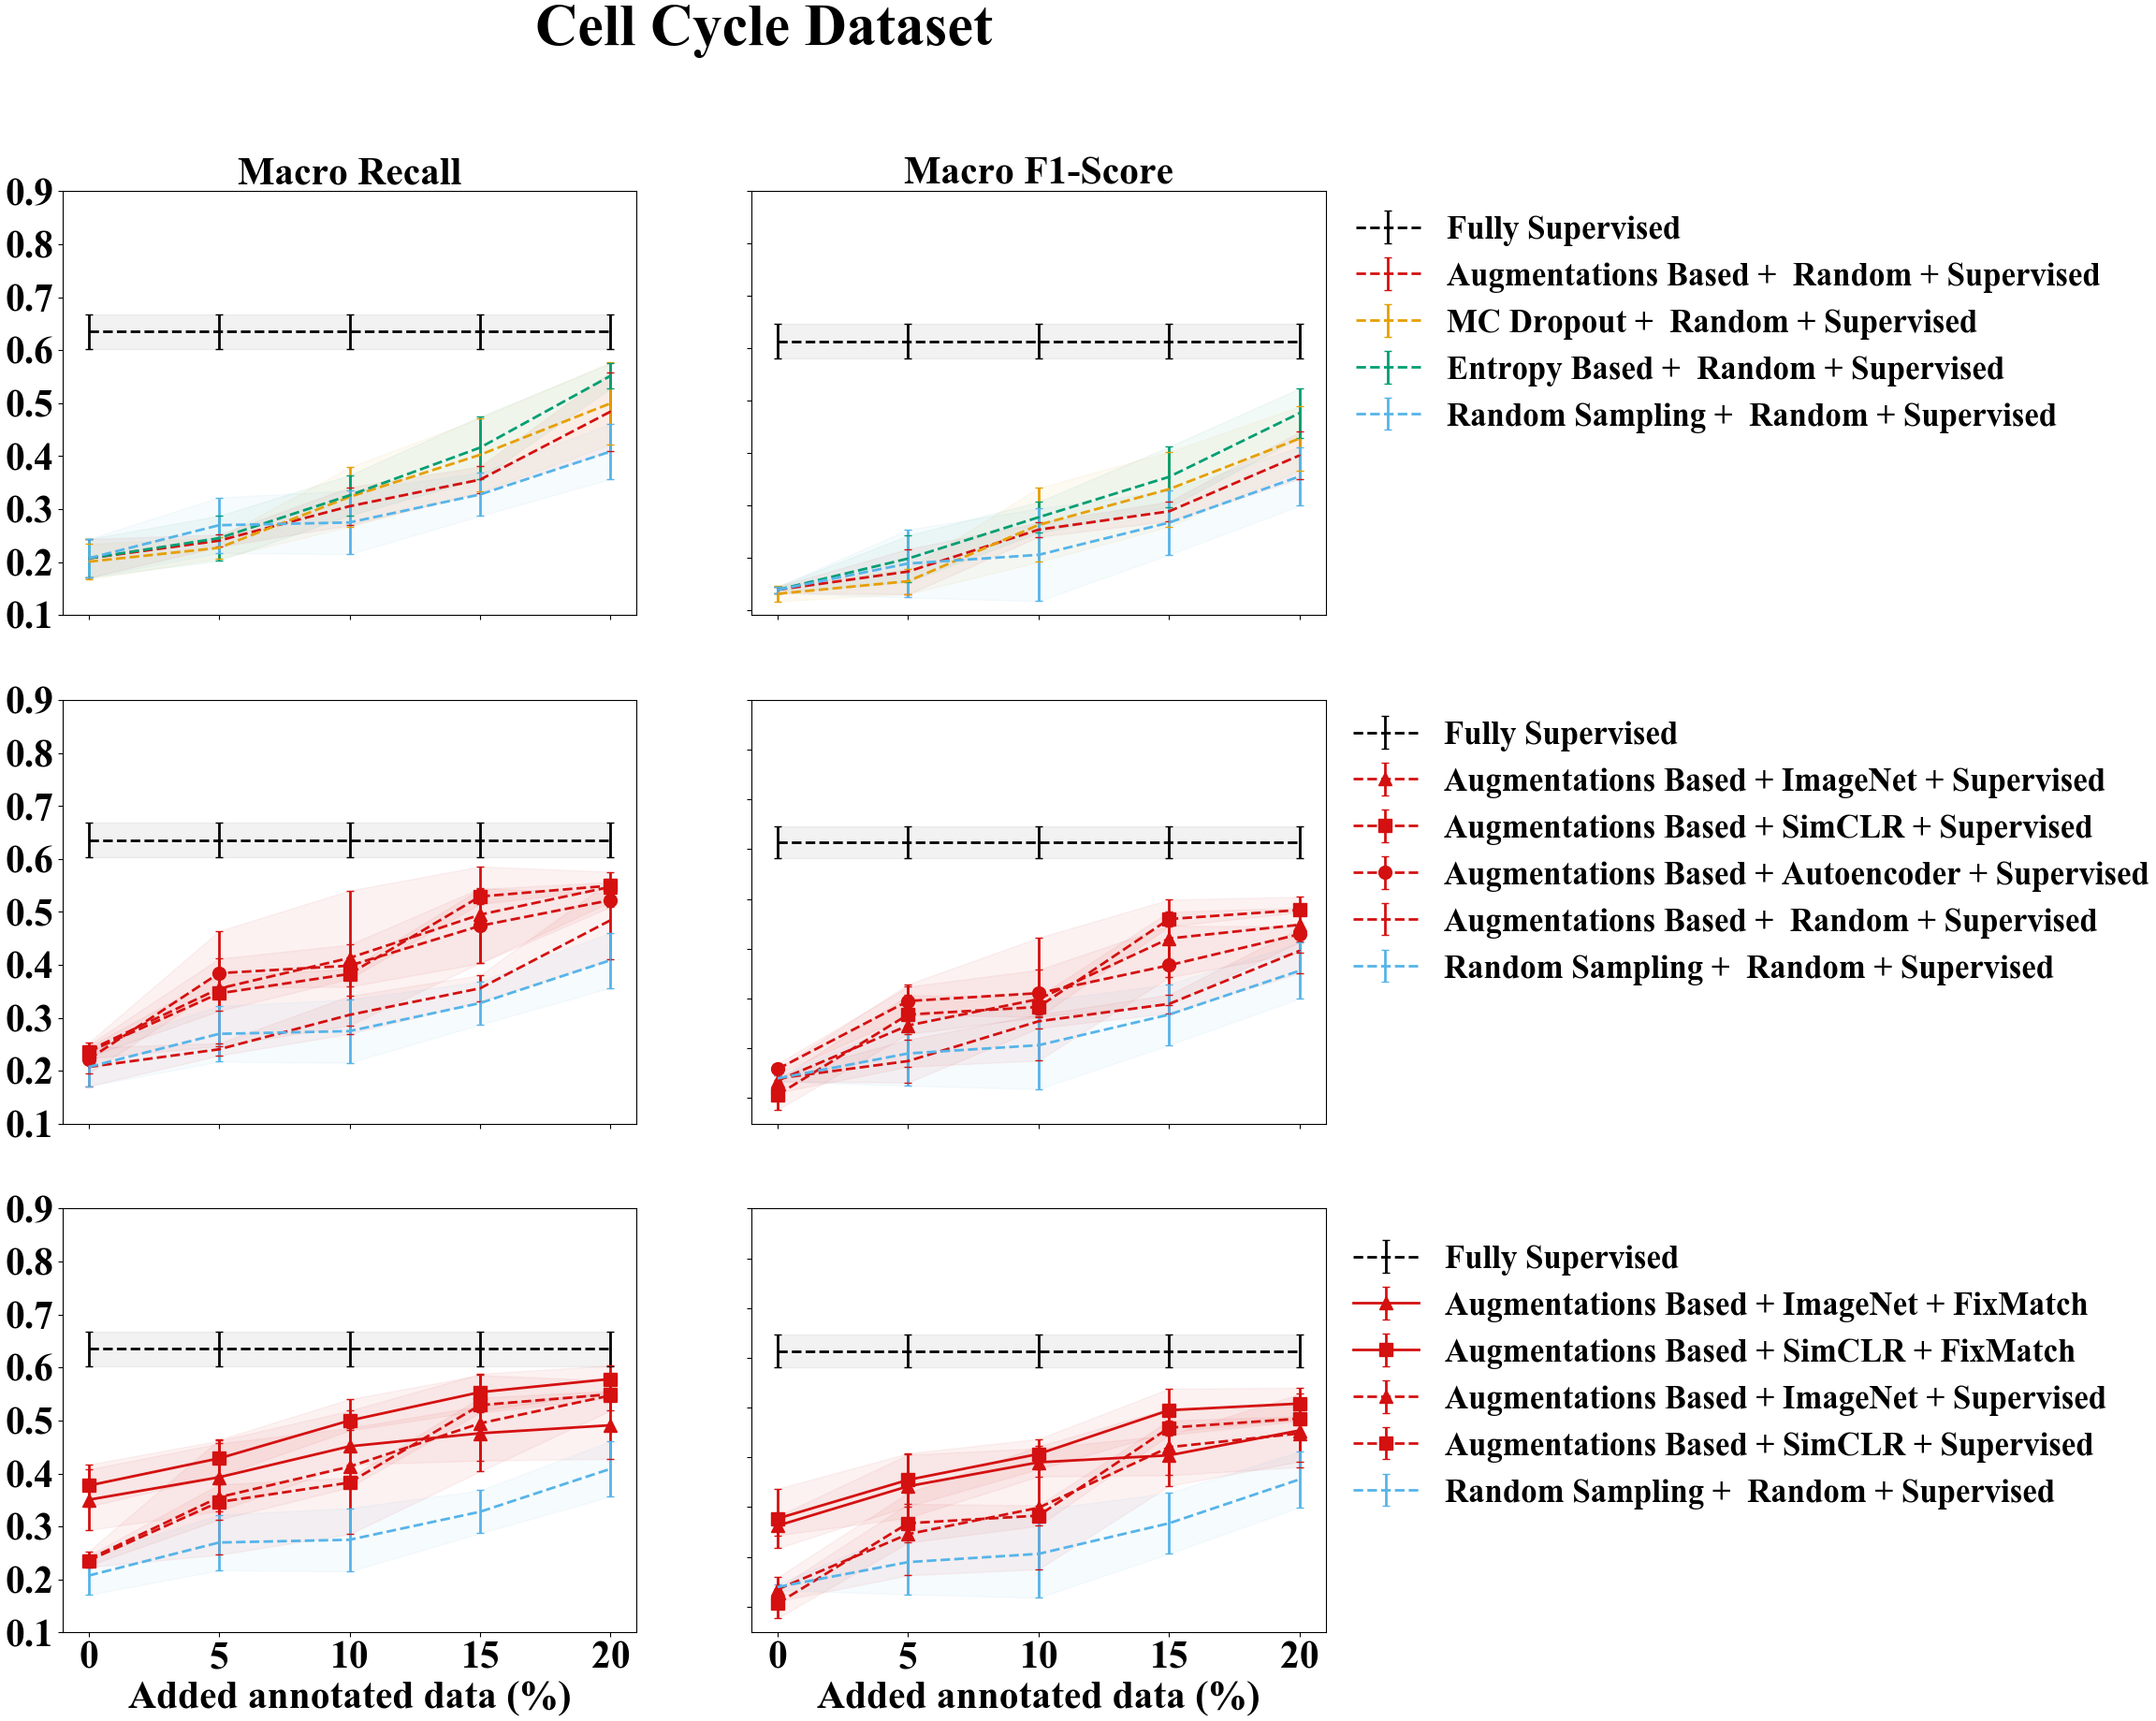
\includegraphics[width=\textwidth]{figures/fig_2_cycle_recall_f1.png}
\caption[Macro recall and macro f1-score on cell cycle dataset]{\textbf{Macro recall and macro f1-score on cell cycle dataset}. In the cell cycle dataset, the combination of augmentation-based sampling, SimCLR pre-training and semi-supervised learning using FixMatch approaches the performance of fully-supervised learning on full dataset. (A) Macro recall and macro f1-score are shown for different active learning algorithms. For cell cycle dataset, entropy-based sampling is the best performing algorithm. MC-dropout and augmentation-based sampling show similar performance. All algorithms perform better than random sampling. (B) Although, entropy-based sampling is the best performing active learning algorithm. It is shown (Table \ref{table:all_experiments_skin}), that augmentation-based sampling performs the best when pre-training and semi-supervised learning is added. Hence, augmentation-based sampling is chosen for showing the effect on performance of using different pre-training methods. (C) FixMatch is added, to test the results after adding semi-supervised learning.}
\label{fig:fig_2_cycle_recall_f1}
\end{figure}

\begin{figure}[htbp]
\centering
\captionsetup{format=plain}
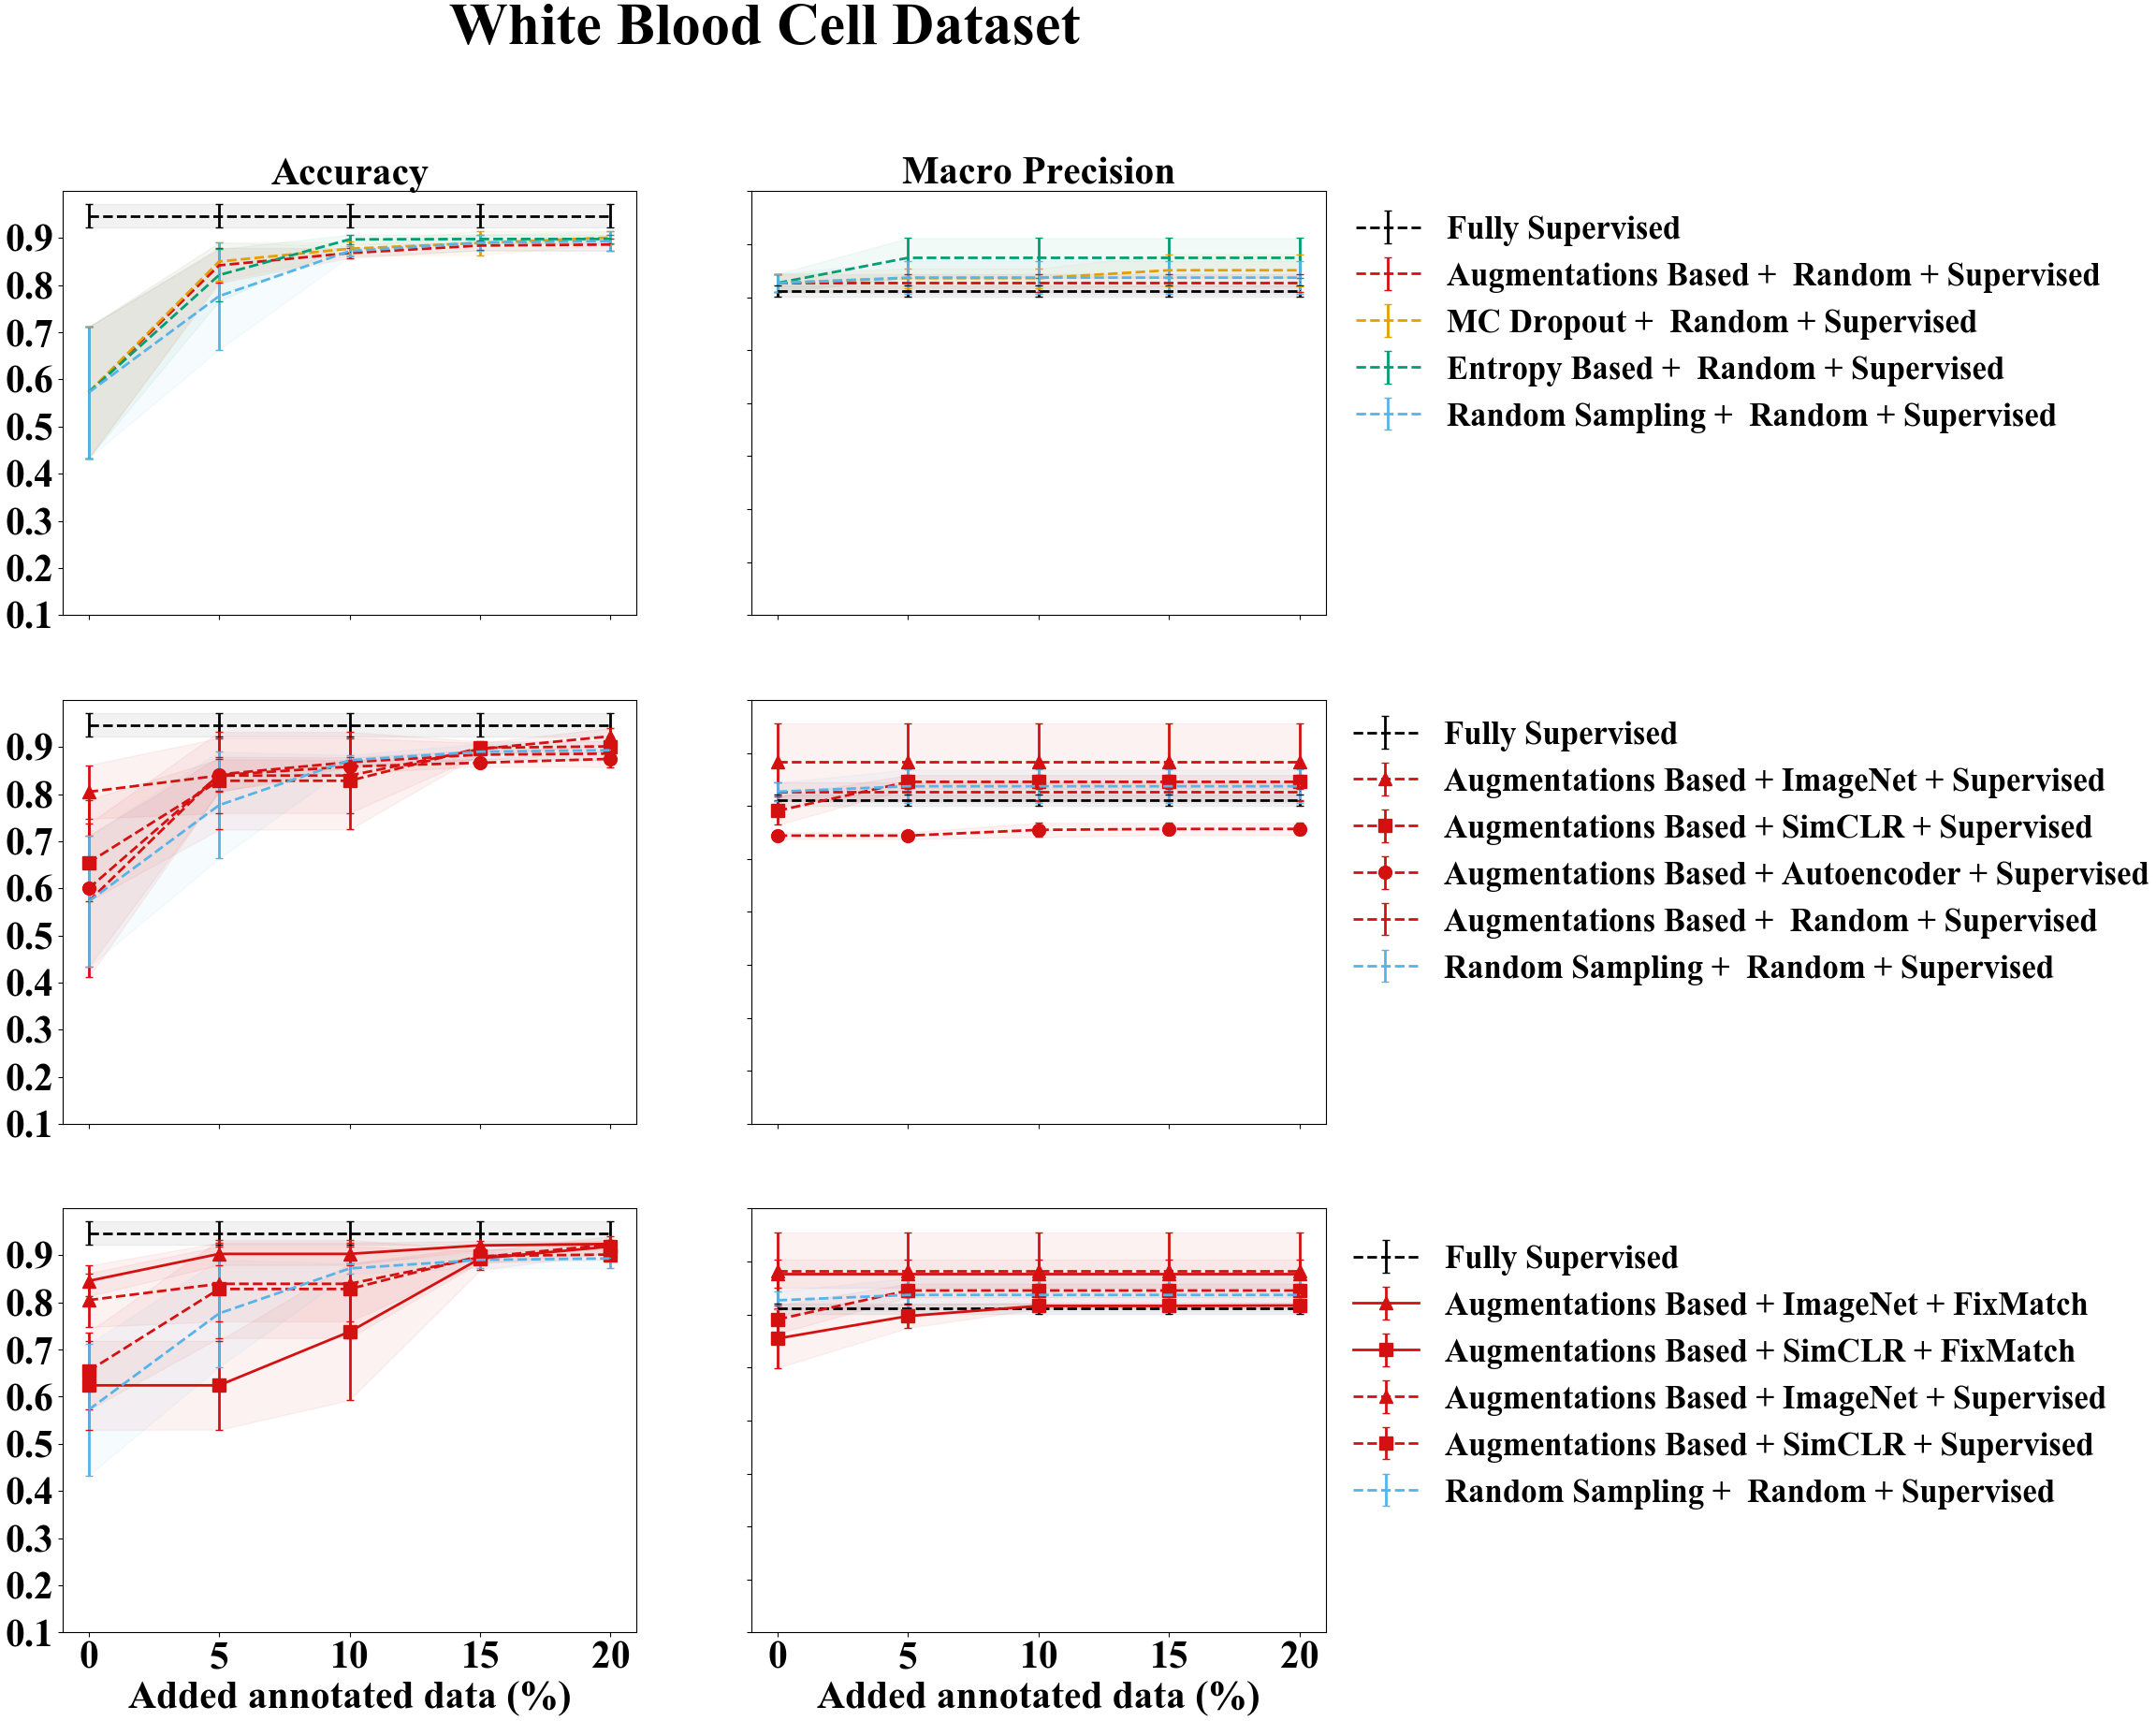
\includegraphics[width=\textwidth]{figures/fig_2_white_acc_precision.png}
\caption[Accuracy and macro precision on white blood cell dataset]{\textbf{Accuracy and macro precision on white blood cell dataset}. On the white blood cell dataset, the combination of augmentation-based sampling, ImageNet pre-training and semi-supervised learning reaches the fully-supervised performance in terms of accuracy. As mentioned in the introductory paragraph of chapter \ref{chapter:results}, macro precision is not a useful metric for the biomedical datasets which are tested in this thesis. (A) Accuracy and macro precision is shown for three active learning algorithms as well as random sampling. (B) Augmentation-based sampling is chosen for further investigation using pre-training methods. The choice is augmentation-based sampling is based on the results of augmentation-based sampling combinations in terms of macro recall (Table \ref{table:all_experiments_skin}). (C) FixMatch is added to record the accuracy and macro precision performance for the combination of augmentation-based sampling, pre-training methods and semi-supervised learning.}
\label{fig:fig_2_white_acc_precision}
\end{figure}

\begin{figure}[htbp]
\centering
\captionsetup{format=plain}
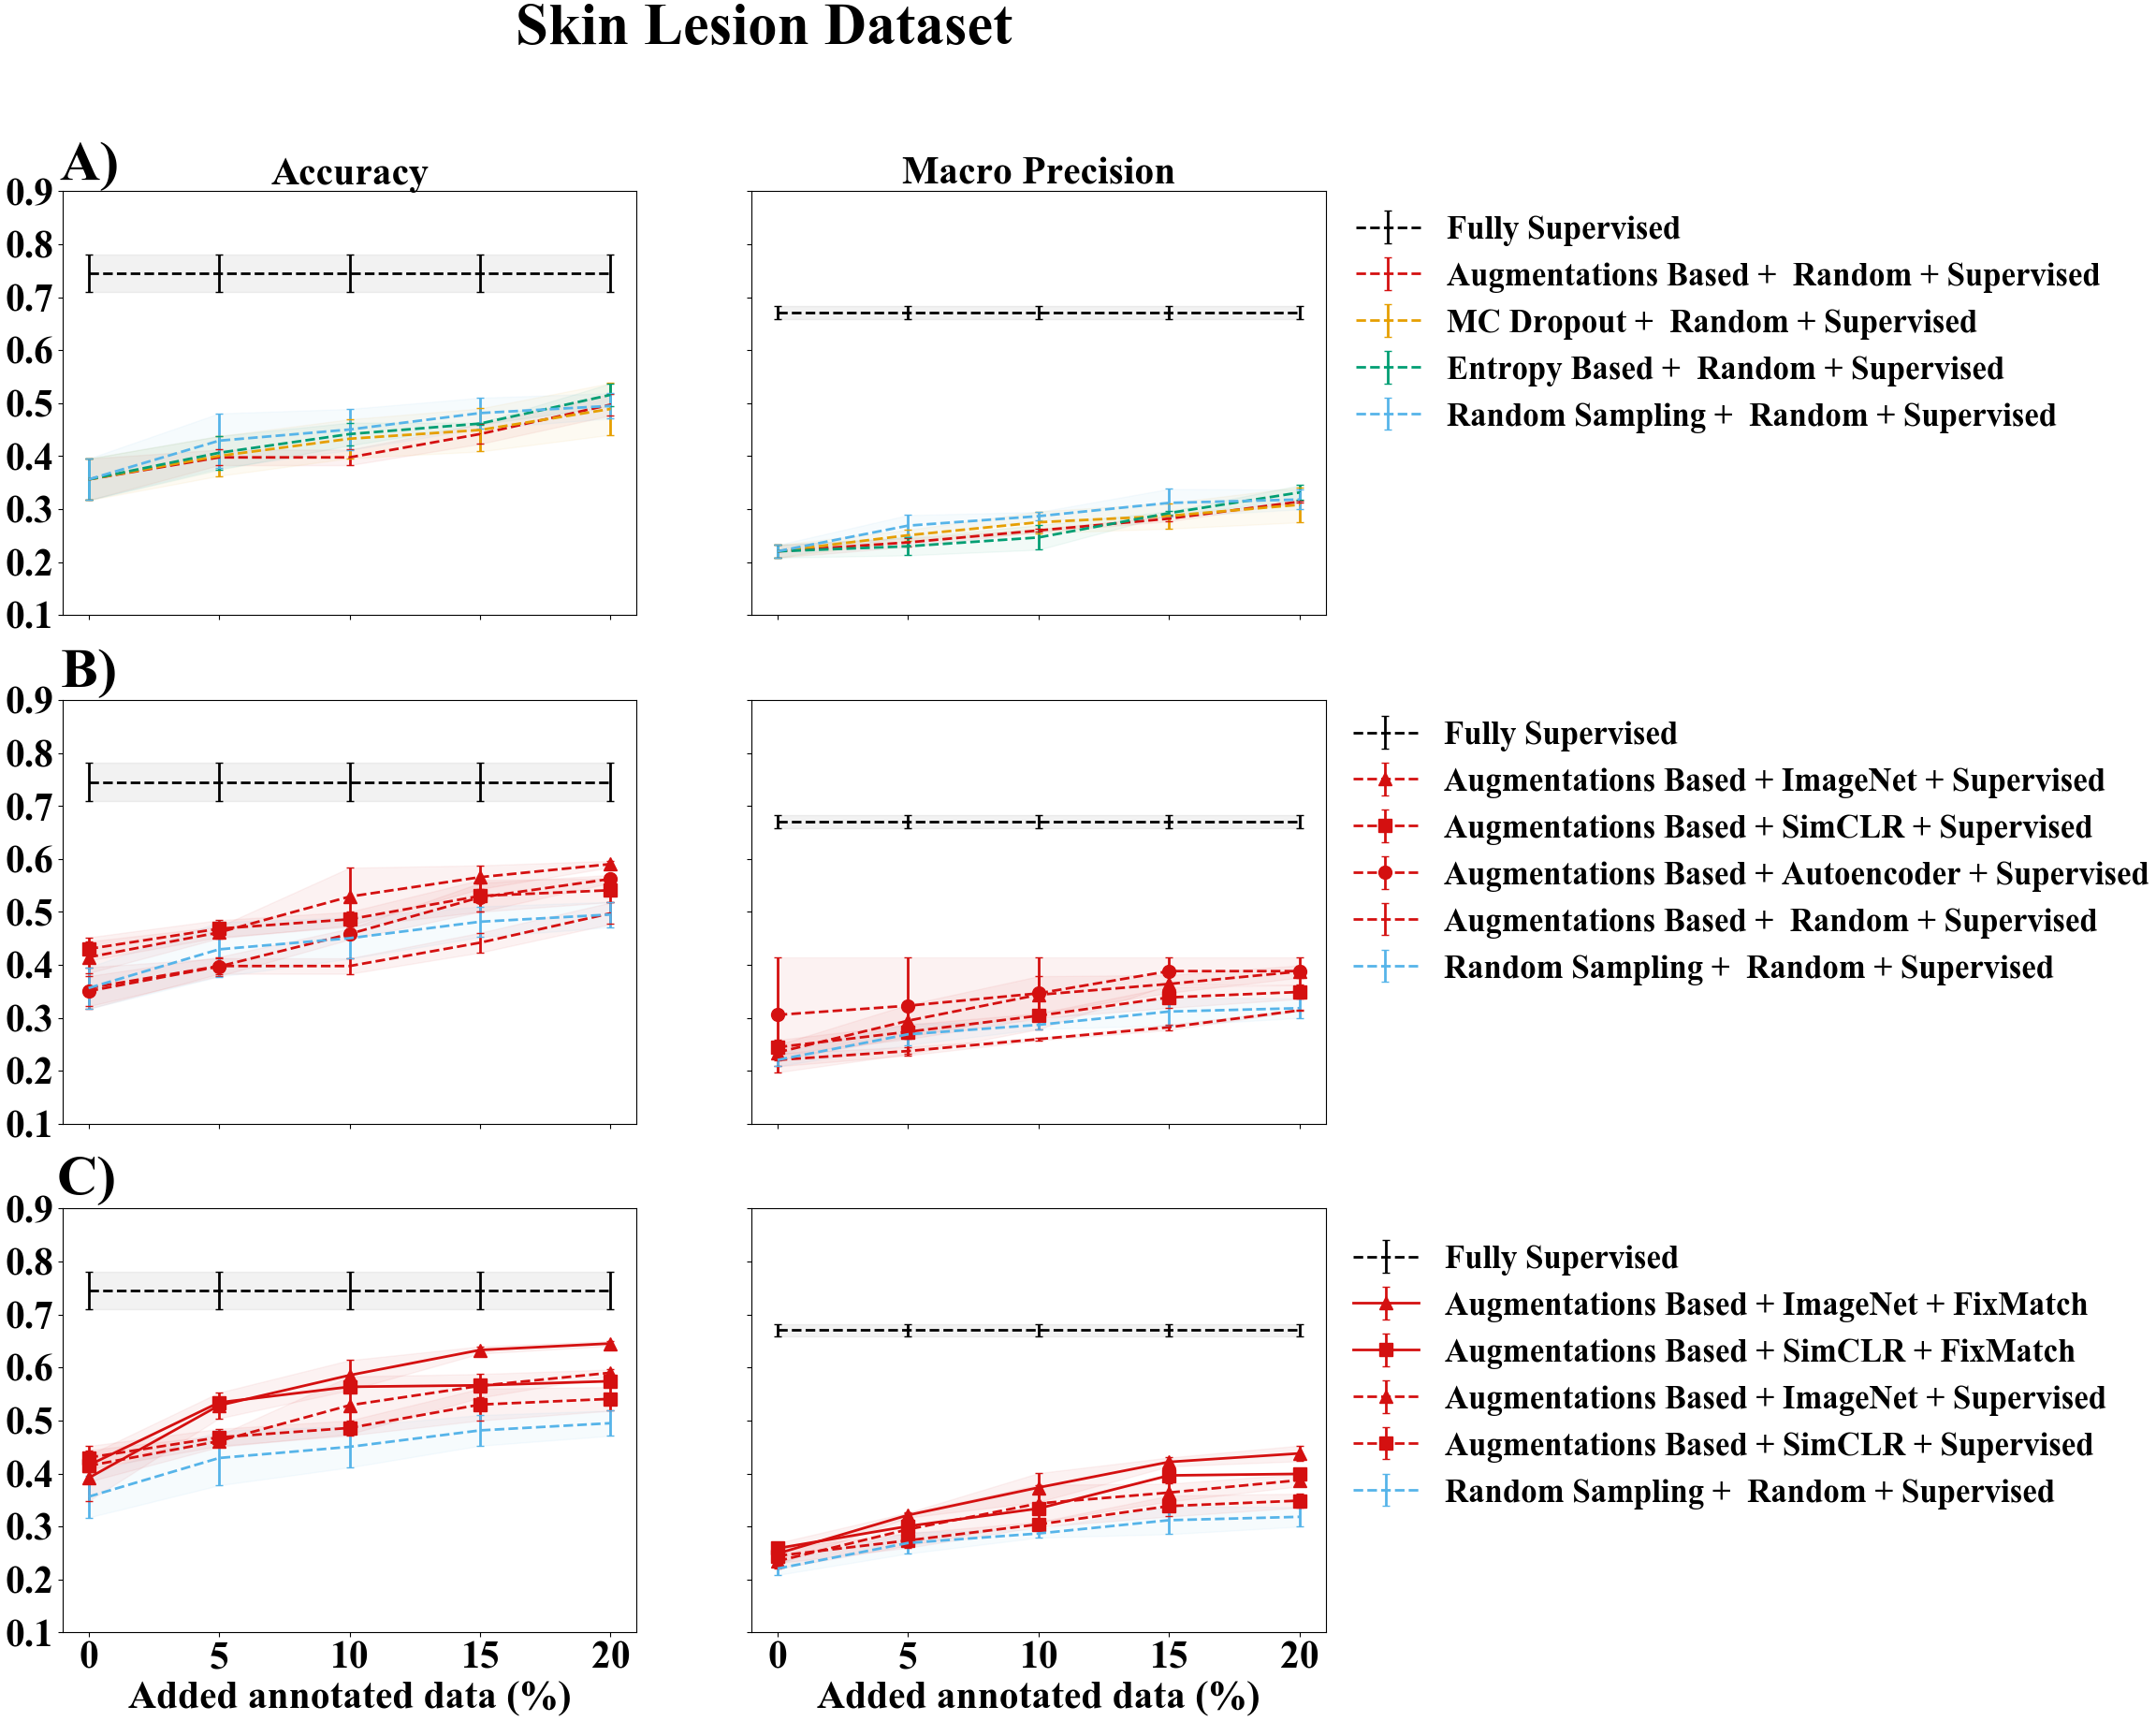
\includegraphics[width=\textwidth]{figures/fig_2_skin_acc_precision.png}
\caption[Accuracy and macro precision on skin lesion dataset]{\textbf{Accuracy and macro precision on skin lesion dataset}. For skin lesion dataset, the combination of augmentation-based sampling, ImageNet pre-training and semi-supervised learning fall short of the accuracy achieved through fully supervised learning. As discussed in the introduction of chapter \ref{chapter:results}, precision does not provide a lot of information regarding the model performance. (A) Accuracy and macro precision has been shown for three active learning algorithms and random sampling. (B) Augmentation sampling is chosen for comparing the performance boost achieved through different pre-training methods. The choice of augmentation-based sampling is made on the basis of its macro recall performance (Table \ref{table:all_experiments_skin}) in combination with ImageNet pre-training and semi-supervised learning. (C) The performance of semi-supervised learning in combination with ImageNet and SimCLR pre-training and augmentation-based sampling is shown.}
\label{fig:fig_2_skin_acc_precision}
\end{figure}

\begin{figure}[htbp]
\centering
\captionsetup{format=plain}
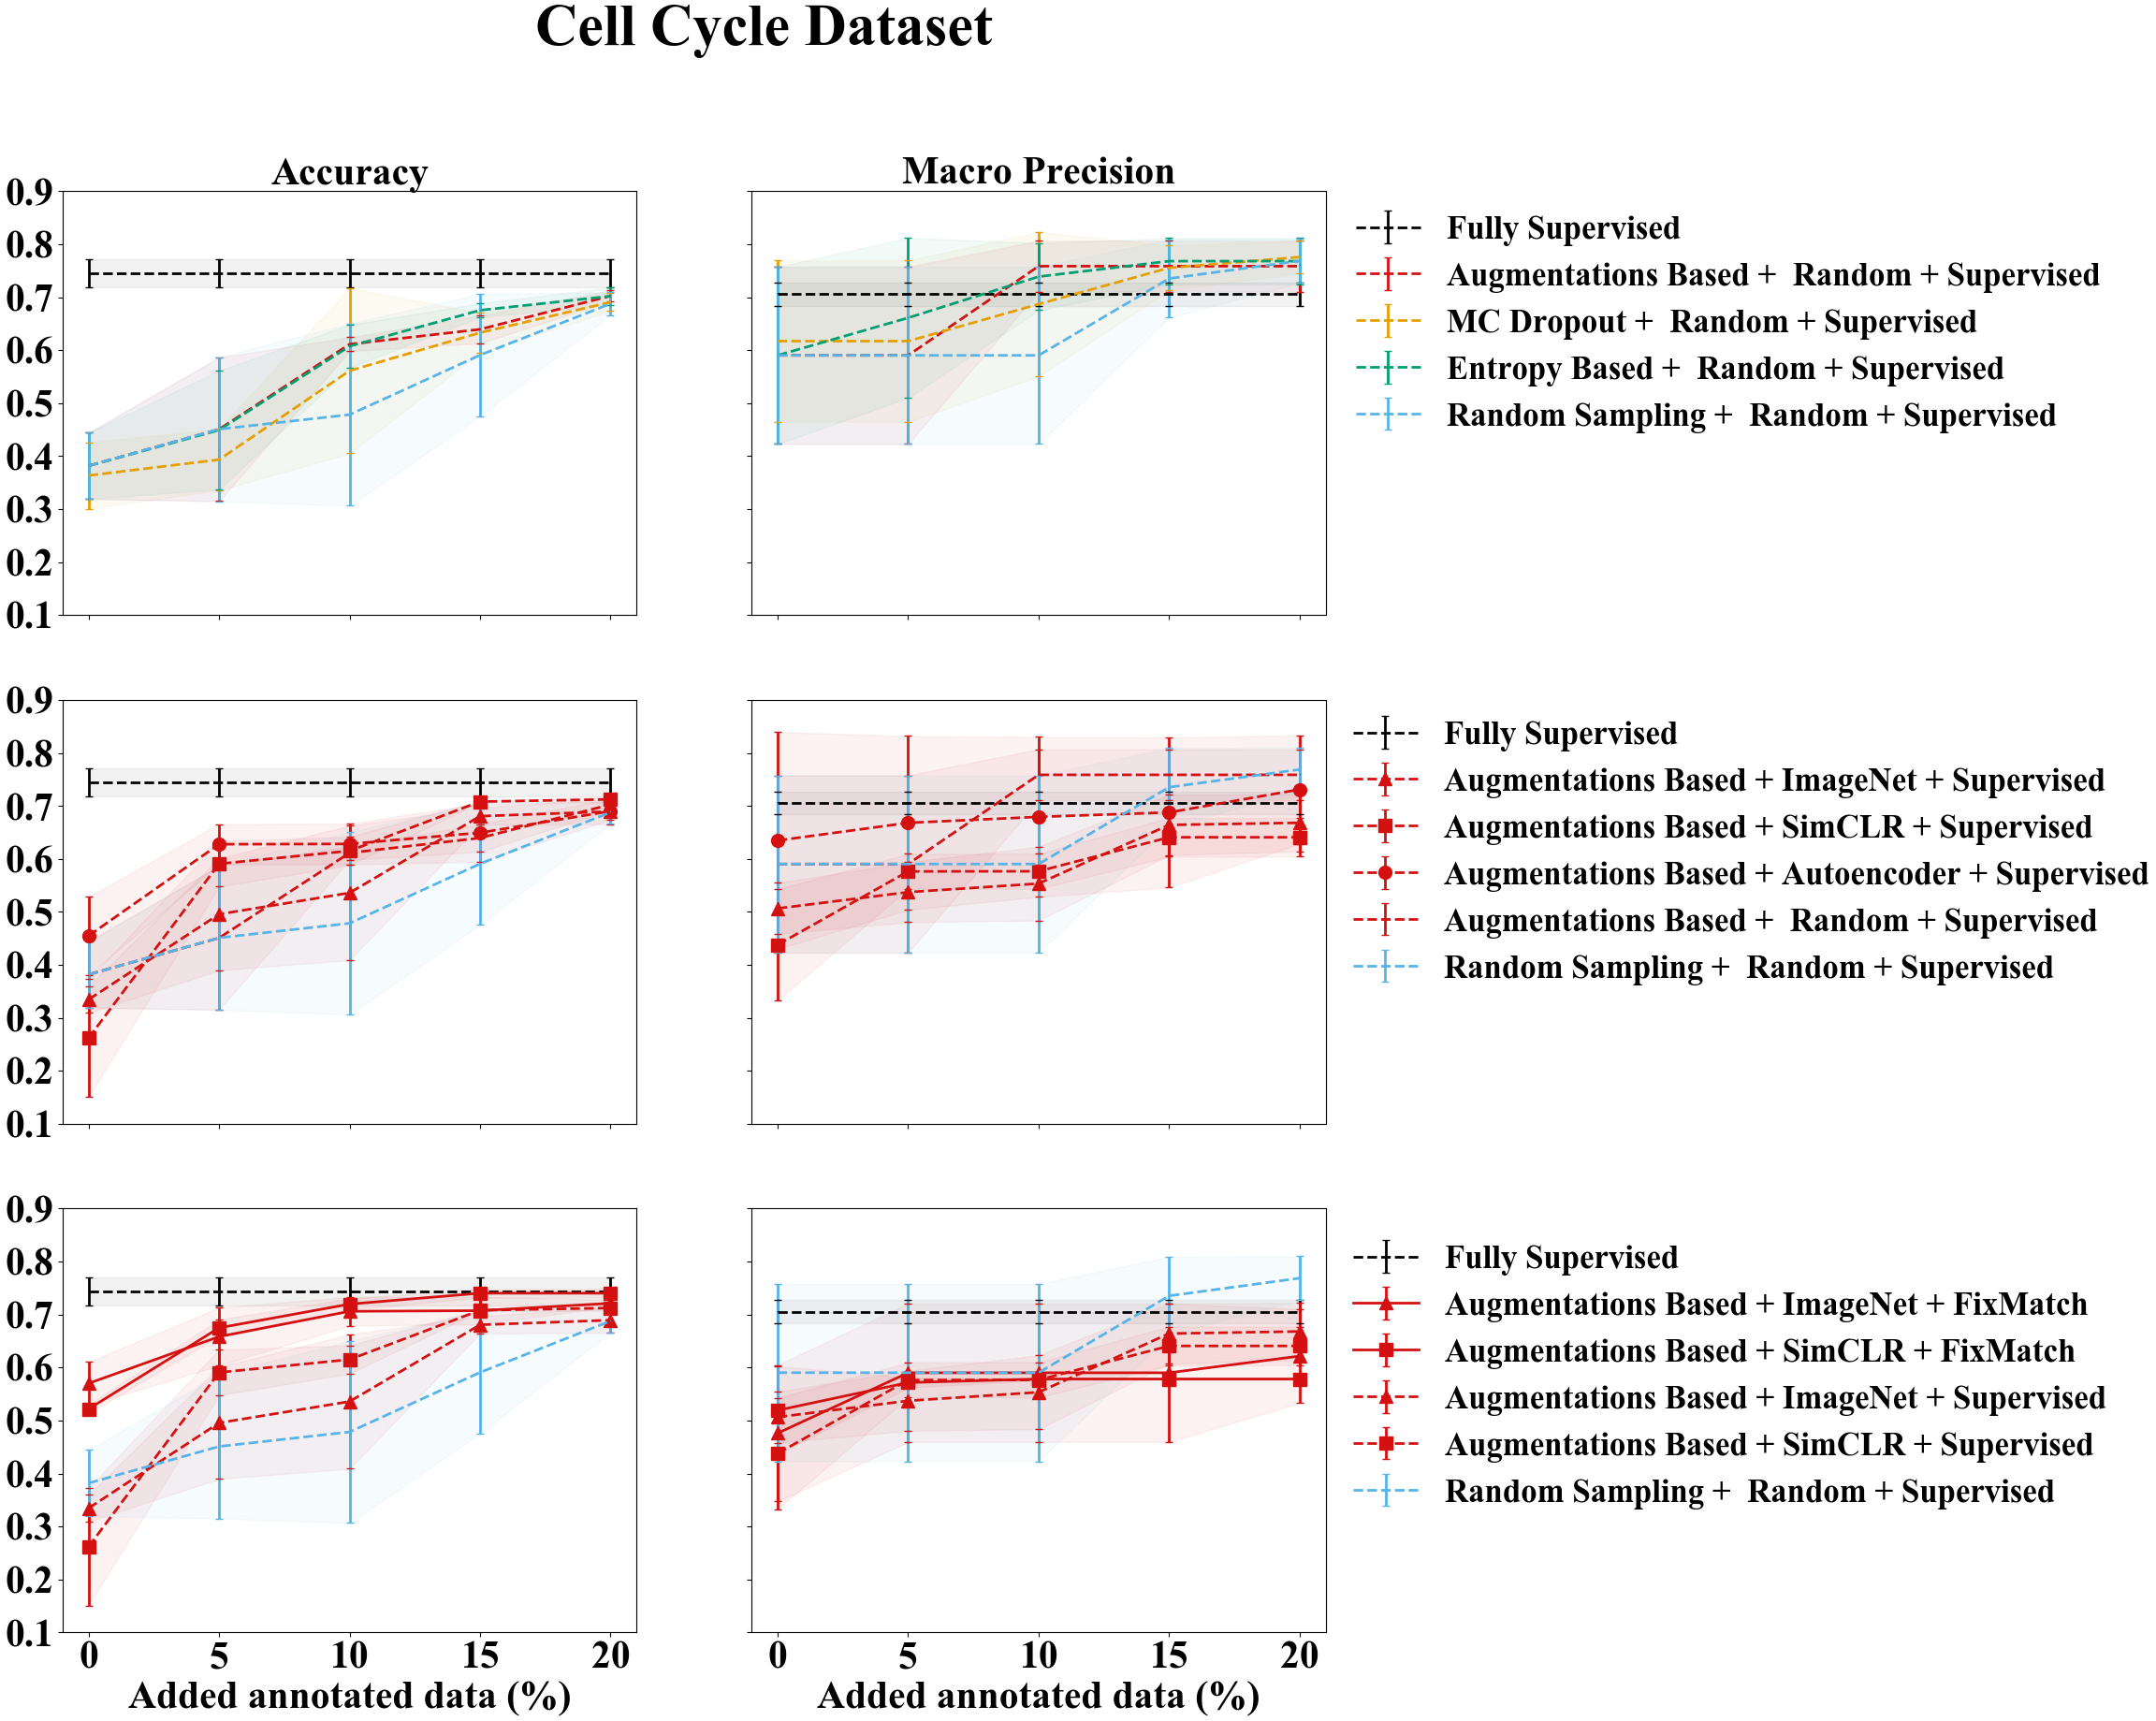
\includegraphics[width=\textwidth]{figures/fig_2_cycle_acc_precision.png}
\caption[Accuracy and macro precision on cell cycle dataset]{\textbf{Accuracy and macro precision on cell cycle dataset}. On cell cycle dataset, the accuracy achieved by the combination of augmentation-based sampling, SimCLR pre-training and semi-supervised learning approaches the accuracy achieved by fully-supervised learning. As discussed in the introductory paragraph of chapter \ref{chapter:results}, macro precision is not expected to act as a good metric for measuring the performance on biomedical datasets tested in this thesis (A) Accuracy and macro precision are measured for the three active learning algorithms as well as random sampling, with random initialization method and supervised training strategy. All active learning algorithms perform similarly. (B) Augmentation-based sampling is chosen for further analysis using three pre-training methods: ImageNet, SimCLR and Autoencoder pre-training. Augmentation-based sampling is chosen because it performs the best for cell cycle dataset when it is tested in combination with SimCLR pre-training and semi-supervised learning (Table \ref{table:all_experiments_skin}). (C) Semi-supervised learning is added and then augmentation-based sampling is tested again with ImageNet and SimCLR pre-training.}
\label{fig:fig_2_cycle_acc_precision}
\end{figure}

\section{Comparison of Active Learning Algorithms on White Blood Cell Dataset}
First, the performance of different label-efficient approaches is compared on the white blood cell dataset (Figure \ref{fig:fig_2_white_recall_f1}). Random initialization is used for model weights initialization and the model is trained under the supervised learning paradigm i.e., using labeled data only. The augmentation-based sampling achieves better performance compared to all other active learning algorithms (Table \ref{table:all_experiments_white}, Table \ref{table:all_experiments_skin}, Table \ref{table:all_experiments_cycle}) in almost all active learning iterations (see Figure \ref{fig:fig_2_white_recall_f1}). At the last active learning iteration, after 20\% of data has already been added to the labeled set $\mathcal{L}$ as labeled images, the augmentation-based sampling has a macro recall of 0.72$\pm$0.03, entropy-based sampling a macro recall of 0.72$\pm$0.02, MC-dropout a recall of 0.66$\pm$0.04 and random sampling a recall of 0.68$\pm$0.02.

\section{Pre-training on White Blood Cell Dataset Further Improves Performance}
Augmentation-based sampling is the best performing active learning algorithm. The performance obtained through augmentation sampling is further improved by adding pre-training (Figure \ref{fig:fig_2_white_recall_f1}). Using augmentation-based sampling as the active learning algorithm, the experiment is repeated with three pre-training methods: using pre-trained ImageNet weights, using Autoencoder and using SimCLR (see chapter \ref{chapter:methods} and Table \ref{table:experimental_grid}). It is found that using pre-trained ImageNet  weights and SimCLR for pre-training results in a boost in performance in the first two active learning iterations with a increase of 12\% of macro recall. However, as more labeled data is added, the random initialization catches up with SimCLR and autoencoder pre-training but ImageNet pre-training still performs better than random initialization even after the addition of 20\% of the data. After the last active learning iteration, the  augmentation-based sampling with ImageNet weights reaches a macro recall of 0.78$\pm$0.03, random initialization reaches a macro recall of 0.72$\pm$0.03 and initialization with SimCLR pre-training reaches a recall of 0.71$\pm$0.04.

\section{Semi-supervised Learning Further Improves Recall for White Blood Cell Dataset}
As augmentation-based sampling performed better than other active learning algorithms, it is chosen for further investigation to find out the performance improvement gained by using semi-supervised learning training strategy (Figure \ref{fig:fig_2_white_recall_f1}). The pre-training methods of using pre-trained ImageNet weights and SimCLR are used, as both of the methods performed well during the previous experiments (Figure \ref{fig:fig_2_white_recall_f1}B). For semi-supervised learning, FixMatch is used (Figure \ref{fig:fig_2_white_recall_f1}C). After adding semi-supervised learning with augmentations, a macro recall improvement of at least 6\% is observed for all iterations. This combination performs better than supervised training in each iteration and achieves a macro recall of 0.82$\pm$0.04 at the last iteration, when 20\% of labeled data has been added to the labeled set $\mathcal{L}$. FixMatch also improves augmentation-based sampling with SimCLR pre-training, reaching 0.79$\pm$0.01 macro recall. It is to be noted that when using augmentation-based active learning algorithm with ImageNet pre-training and semi-supervised learning, the macro recall is only 4\% less than using fully-supervised learning on 100\% of the data.

\section{Grid-search Identifies the Best Performing Combinations for Three Biomedical Datasets}
To investigation if the proposed combination of augmentation-based sampling, ImageNet pre-training and semi-supervised learning performs better than other combinations in table \ref{table:experimental_grid} for biomedical datasets which involve images containing different textures, colors and structures. The proposed combination is tested on three different biomedical datasets (Figure \ref{fig:datasets_composition}). For this purpose an extensive grid search is carried out which specifically involves, 3x4x4x2x4x5 = 1920 independent runs (3 datasets, 3 active learning algorithms plus random sampling, 3 pre-training methods plus random initialization, 2 training strategies, 4-fold cross-validation and 1 initial step plus 4 active learning iterations). The criteria for measuring the performance of different combinations is the macro recall value at the last iteration when 20\% of data has been added as labeled data.

It is found that the proposed combinations of augmentation-based sampling with ImageNet or SimCLR pre-training and FixMatch consistently outperform the rest (for comparing all the combinations, please refer to the appendix).
In the white blood cell dataset, at the first step with 1\% of labeled data a 6\% improvement in macro recall at least is observed using FixMatch with ImageNet initialization over conventional training method with only labeled data (Figure \ref{fig:all_recall_f1}A). This improvement in performance is stable, resulting in at least 4\% increase in macro recall compared to the best result obtained through supervised learning training strategy. The same trend is observed in the skin lesion dataset (Figure \ref{fig:all_recall_f1}B). During the first iteration, an improvement of at least 5\% is observed compared to other supervised learning conventional methods. Although the conventional supervised learning methods approach the performance of proposed combinations as more data is added, there is still a performance gap at all iterations. Lastly, for the cell cycle dataset (Figure \ref{fig:all_recall_f1}C), the combination of SimCLR with augmentation-based sampling provides a boost of at least 16\% in the macro recall in the start over other conventional methods. The performance boost gets less as more data is added but till the last iteration when 20\% of data has been added as labeled data, the performance improvement is still at least 3\% of macro recall. 
It is to be noted that, at the last iteration, for white blood cell dataset and the cell cycle dataset, the performance of the propose combinations approach the performance of fully-supervised learning on the whole dataset. However, in the skin lesion dataset, more labeled data has to be added to approach the performance of fully supervised learning. 

\begin{figure}[htbp]
\centering
\captionsetup{format=plain}
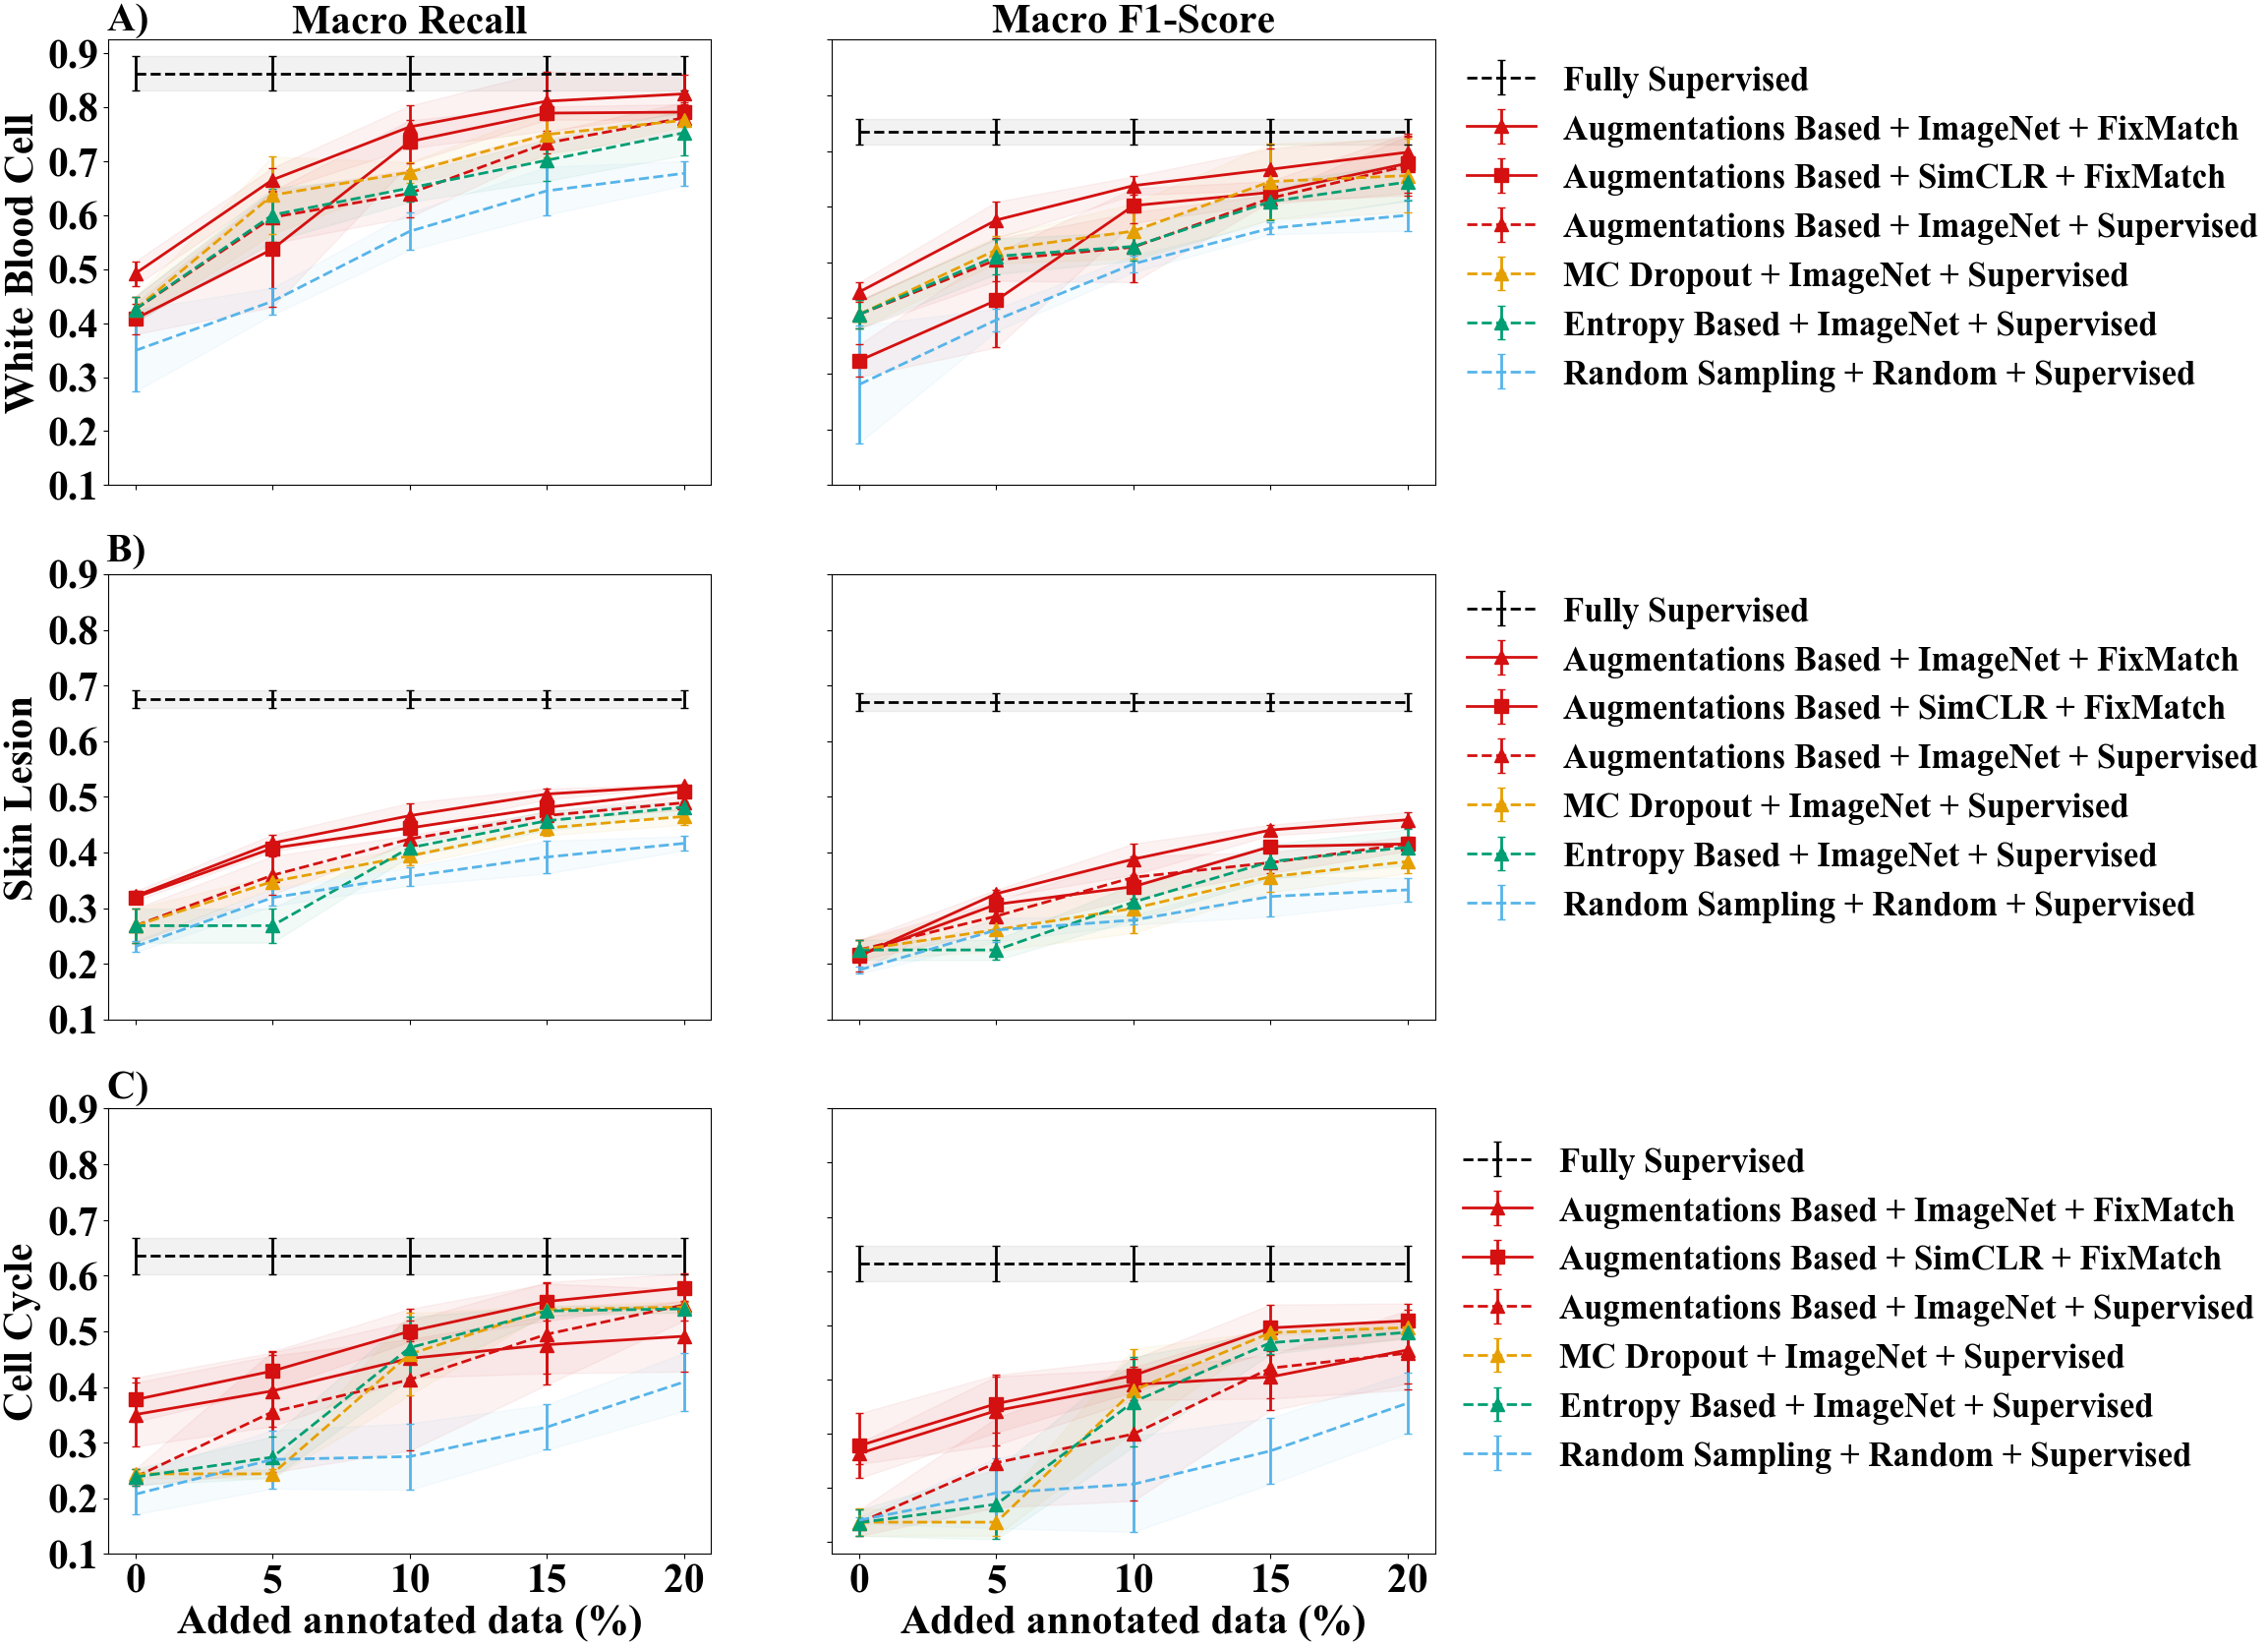
\includegraphics[width=\textwidth]{figures/fig_3_recall_f1.png}
\caption[Macro recall and macro f1-score on all datasets]{\textbf{Macro recall and macro f1-score on all datasets}. On all datasets, the combination of augmentation-based sampling, SimCLR pre-training and semi-supervised learning performs the best in terms of macro recall or macro f1-score. The optimal combination with ImageNet pre-training performs better than other combinations on white blood cell and skin lesion datasets. (A) For white blood cell dataset, the optimal combination outperforms all the conventional baseline combinations on each active learning iteration for macro recall and macro f1-score. The optimal combination was at least 3\% better then combinations for macro recall and at least 2\% better for macro f1-score. (B) On skin lesion dataset, the optimal combination outperforms all conventional combinations at each active learning iteration for macro recall and on all active learning iterations except the first one for macro f1-score (C) For cell cycle dataset, the optimal combination of augmentation-based sampling, SimCLR pre-training and semi-supervised learning performs better than all combinations but using ImageNet pre-training rather than SimCLR results in a performance degradation.}
\label{fig:all_acc_precision}
\end{figure}

\begin{figure}[htbp]
\centering
\captionsetup{format=plain}
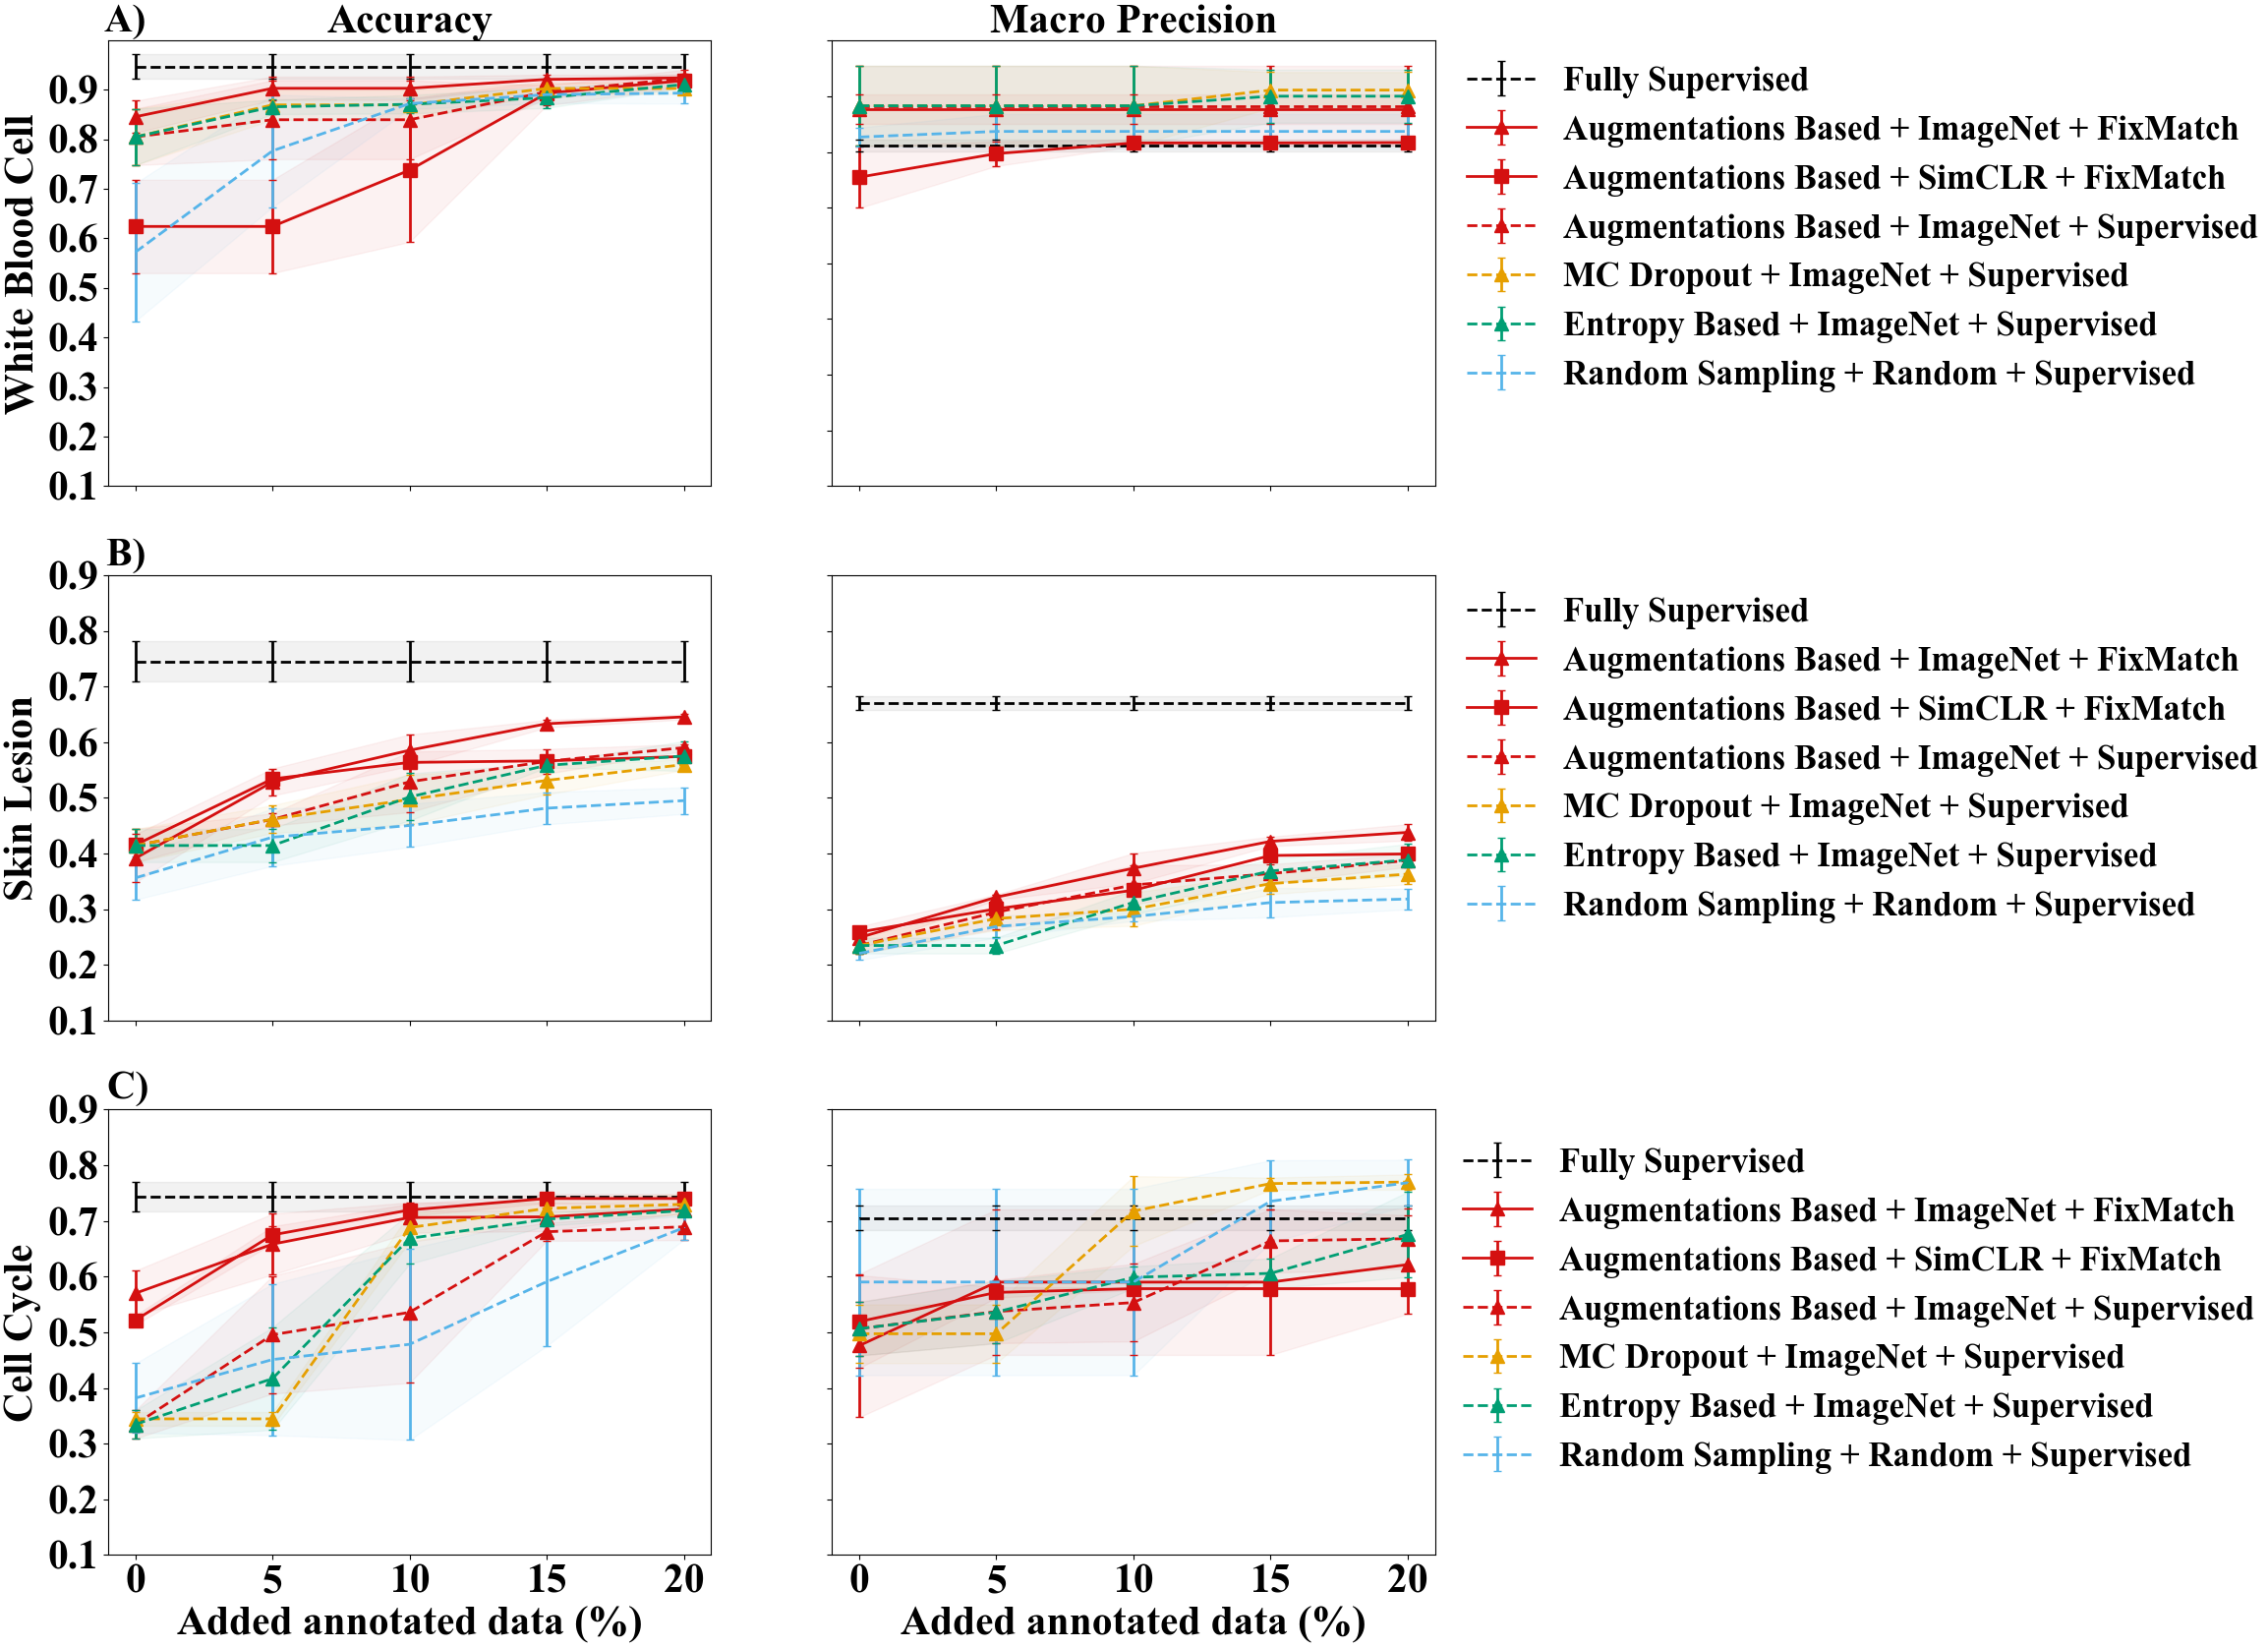
\includegraphics[width=\textwidth]{figures/fig_3_acc_precision.png}
\caption[Accuracy and macro precision on all datasets]{\textbf{Accuracy and macro precision on all datasets}. Augmentation-based sampling, SimCLR or ImageNet pre-training and semi-supervised learning using FixMatch is the optimal combination for accuracy on all datasets. However, for macro precision, as mentioned in the introduction of chapter \ref{chapter:results}, the values of macro precision do not provide a good measurement of how good the model is performing for the biomedical datasets being tested in this thesis.}
\label{fig:all_recall_f1}
\end{figure}

\newpage

\section{Recommended Strategy}
As a result of the previous sections, the optimal strategy is identified as the combination of augmentation-based sampling, ImageNet/SimCLR pre-training and FixMatch to show the best results on 3 biomedical datasets. As illustrated in Figure 3, the ImageNet pre-training works better for white blood cell dataset and the skin lesion dataset from the initial step. SimCLR pre-training seems to work best on the cell cycle data. Therefore, the recommended strategy is to find the best pre-training method on the initial step and combine it with augmentation-based sampling and FixMatch during training. The results of the recommended strategy improves macro recall by 4\% for white blood cell dataset, 3\% on skin lesions data and 3\% for cell cycle data on the last iteration, with respect to the best conventional active learning method for each dataset.


\begin{sidewaystable}[htbp]
\captionsetup{format=plain}
\centering
 \begin{tabular}{c c c c c c c c} 
 \hline
 A & \thead{Active \\ learning \\ algorithm} & \thead{Pre-\\training \\ method} & \thead{Training \\ strategy} & \thead{Accuracy} & \thead{Precision} & \thead{Recall} & \thead{F1-score} \\ [0.5ex] 
 \hline
 Fully-supervised & - & 
 ImageNet & 
 \makecell{Supervised\\learning} & 
 0.95±0.02 & 0.71±0.01 & 0.86±0.03 & 0.73±0.02 \\
 \hline
 \textbf{Recommended} & \makecell{Augmentation\\-based} & ImageNet & 
 FixMatch & \textbf{0.92±0.02} & 0.78±0.07 & \textbf{0.82±0.04} & \textbf{0.70±0.03}
  \\
 \makecell{Conventional\\(baseline)} & \makecell{Augmentation\\-based} &
 ImageNet & 
 \makecell{Supervised\\learning} & 0.92±0.02 & 0.78±0.07 & 0.78±0.03 & 0.67±0.05
  \\
 \makecell{Conventional\\(baseline)} & MC-dropout & 
 ImageNet & 
 \makecell{Supervised\\learning} & 0.90±0.01 & \textbf{0.81±0.03} & 0.78±0.01 & 0.66±0.07
  \\
 \makecell{Conventional\\(baseline)} & \makecell{Entropy\\-based} & 
 ImageNet & 
 \makecell{Supervised\\learning} & 0.91±0.01 & 0.8±0.05 & 0.75±0.04 & 0.64±0.03 \\
 \hline
 \makecell{No active\\learning} & Random & 
 Random & 
 \makecell{Supervised\\learning} & 
 0.89±0.02 & 0.74±0.03 & 0.68±0.02 & 0.58±0.03 \\
 \hline
\end{tabular}
\caption[Accuracy, macro precision, macro recall and macro f1-score for white blood cell dataset]{\textbf{Accuracy, macro precision, macro recall and macro f1-score for white blood cell dataset}. Comparing the results of the last iteration, the recommended strategies outperform conventional label-efficient learning. (A) On the white blood cell dataset, the combination of augmentation-based sampling, ImageNet pre-training and FixMatch training brings an improvement of 4\% on macro recall and 3\% on F1-score over the highest baseline. With using only 20\% of added labeled data, this strategy is only 4\% lower in recall and 3\% lower with respect to the F1-score as compared to fully-supervised training.}
\label{table:all_experiments_white}
\end{sidewaystable}

\begin{sidewaystable}[htbp]
\captionsetup{format=plain}
\centering
 \begin{tabular}{c c c c c c c c} 
 \hline
 B & \thead{Active \\ learning \\ algorithm} & \thead{Pre-\\training \\ method} & \thead{Training \\ strategy} & \thead{Accuracy} & \thead{Precision} & \thead{Recall} & \thead{F1-score} \\ [0.5ex] 
 \hline
 Fully-supervised & - & 
 ImageNet & 
 \makecell{Supervised\\learning} & 
 0.75±0.04 & 0.67±0.01 & 0.68±0.02 & 0.67±0.02 \\
 \hline
 \textbf{Recommended} & \makecell{Augmentation\\-based} & ImageNet & 
 FixMatch & 
 \textbf{0.65±0.00} & 0.44±0.01 & \textbf{0.52±0.00} & \textbf{0.46±0.01} \\
 \makecell{Conventional\\(baseline)} & \makecell{Augmentation\\-based} &
 ImageNet & 
 \makecell{Supervised\\learning} & 
 0.59±0.01 & 0.39±0.01 & 0.49±0.01 & 0.42±0.01 \\
 \makecell{Conventional\\(baseline)} & \makecell{Entropy\\-based} & 
 ImageNet & 
 \makecell{Supervised\\learning} & 
 0.58±0.03 & \textbf{0.39±0.03} & 0.48±0.01 & 0.41±0.03 \\
 \makecell{Conventional\\(baseline)} & MC-dropout & 
 ImageNet & 
 \makecell{Supervised\\learning} & 
 0.56±0.01 & 0.36±0.02 & 0.46±0.01 & 0.38±0.02 \\
 \hline
 \makecell{No active\\learning} & Random & 
 Random & 
 \makecell{Supervised\\learning} & 
 0.50±0.02 & 0.32±0.02 & 0.42±0.01 & 0.33±0.02  \\
 \hline
 \hline
\end{tabular}
\caption[Accuracy, macro precision, macro Recall and macro f1-score for skin lesion dataset]{\textbf{Accuracy, macro precision, macro Recall and macro f1-score for skin lesion dataset}. Comparing the results of the last iteration, the recommended strategies outperform conventional label-efficient learning. (B) On the skin lesions dataset, the recommended strategy brings an improvement of 3\% on macro recall, 5\% improvement on precision and 6\% on F1-score. The high recall difference to the fully-supervised results shows that the amount of labeled data was not enough and more iterations were needed.}
\label{table:all_experiments_skin}
\end{sidewaystable}

\begin{sidewaystable}[htbp]
\captionsetup{format=plain}
\centering
 \begin{tabular}{c c c c c c c c} 
 \hline
 C & \thead{Active \\ learning \\ algorithm} & \thead{Pre-\\training \\ method} & \thead{Training \\ strategy} & \thead{Accuracy} & \thead{Precision} & \thead{Recall} & \thead{F1-score} \\ [0.5ex] 
 \hline
 Fully-supervised & - & 
 ImageNet & 
 \makecell{Supervised\\learning} & 
 0.74±0.03 & 0.71±0.02 & 0.64±0.03 & 0.61±0.03 \\
 \hline
 \textbf{Recommended} & \makecell{Augmentation\\-based} & SimCLR & 
 FixMatch & 
 \textbf{0.74±0.01} & 0.58±0.00 & \textbf{0.58±0.03} & \textbf{0.51±0.03} \\
 \makecell{Conventional\\(baseline)} & \makecell{Augmentation\\-based} &
 ImageNet & 
 \makecell{Supervised\\learning} & 
 0.69±0.02 & 0.67±0.05 & 0.55±0.03 & 0.45±0.06 \\
 \makecell{Conventional\\(baseline)} & MC-dropout & 
 ImageNet & 
 \makecell{Supervised\\learning} & 
 0.73±0.02 & \textbf{0.77±0.01} & 0.54±0.01 & 0.50±0.01 \\
 \makecell{Conventional\\(baseline)} & \makecell{Entropy\\-based} & 
 ImageNet & 
 \makecell{Supervised\\learning} & 
 0.72±0.01 & 0.68±0.08 & 0.54±0.01 & 0.49±0.01 \\
 \hline
 \makecell{No active\\learning} & Random & 
 Random & 
 \makecell{Supervised\\learning} & 
 0.69±0.02 & 0.77±0.04 & 0.41±0.05 & 0.36±0.06  \\
 \hline
 \hline
\end{tabular}
\caption[Accuracy, macro precision, macro recall and macro f1-score for cell cycle dataset]{\textbf{Accuracy, macro precision, macro recall and macro f1-score for cell cycle dataset}. Comparing the results of the last iteration, the recommended strategies outperform conventional label-efficient learning. (C) On the cell cycle dataset, the recommended strategy brings an improvement of 3\% on recall and 6\% on F1-score.}
\label{table:all_experiments_cycle}
\end{sidewaystable}